\documentclass {article}

\usepackage[T1]{fontenc}
\usepackage[english]{babel}
\usepackage{amsmath}
\usepackage{bbm}
\usepackage{listings}
\usepackage{array}
\usepackage{booktabs}
\usepackage{varioref}
\usepackage{indentfirst}
\usepackage{newclude}
\usepackage{lmodern}
\usepackage{algorithmicx}
\usepackage{algorithm}
\usepackage{eurosym}
\usepackage{algpseudocode}
\usepackage{amsthm}
\usepackage{url}
\usepackage{mathrsfs}
\usepackage{fullpage}
\usepackage[utf8]{inputenc}
\usepackage[left=3cm,right=3cm,top=1cm,bottom=2cm]{geometry}
\usepackage{libertine}
\usepackage[pdftex]{graphicx}
\usepackage{wallpaper}
\usepackage{amssymb}
\usepackage{transparent}
\usepackage{eso-pic}
\usepackage{hyperref}
\usepackage{float}
\usepackage{fancyhdr}
\usepackage{lastpage}
\usepackage{titlesec}
\usepackage{caption}
\usepackage[framemethod=default]{mdframed}

\hypersetup
{
    colorlinks = true,
    linkbordercolor = {blue}
}

\geometry{headsep=5ex}
\pagestyle{fancy}
\fancyfoot[C]{\textbf{page \thepage}}
\fancyhead[L]{\textbf{Automatic Differentiation}}
\fancyhead[R]{\rightmark}
\counterwithout{figure}{part}

\renewcommand{\headrulewidth}{1pt}
\renewcommand{\thefigure}{\arabic{part}.\arabic{figure}}
\renewcommand{\footrulewidth}{1pt}
\newcommand{\HRule}{\rule{\linewidth}{0.5mm}}

\newmdenv[linecolor=red, linewidth=1]{frameth}
\newmdenv[linecolor=green, linewidth=1]{framedef}

\begin{document}

	\begin{titlepage}
					
		\vspace*{\stretch{1}}
		\begin{center}
			 	\HRule \\ [0.6cm]
    				\Huge {GREEKS COMPUTATION WITH AUTOMATIC DIFFERENTIATION} \\ [0.4cm] 
				\HRule \\[0.4cm]
		\end{center}
		\vspace*{\stretch{1}}
		
		\begin{figure}
			\begin{minipage}{0.4\textwidth}
				
\includegraphics[scale = 0.09]{LogoSorbonne.png}
			\end{minipage}
			\hspace{19ex}
			\begin{minipage}{0.4\textwidth}
				
\includegraphics[scale = 0.7]{LogoX.png}				
			 \end{minipage}
		\end{figure}

		\begin{center}
			\Huge{\textsc{MSc. Probability \& Finance} \\
			\Huge{\textit{Numerical Probability Project}}} \\
			\bigbreak
			\LARGE{Feb. - Apr. 2020}
		\end{center}
		\vspace*{\stretch{1}}
		
		\begin{minipage}[c]{12cm}
			\bigbreak
			\bigbreak
			\bigbreak
			\bigbreak
			\bigbreak
			\bigbreak
			\bigbreak
			\huge{\textbf{Author}} \\
			\LARGE{Matthieu CHARRIER} \\
			\textit{Student at MSc. Probability \& Finance} \\
			\underline{matthieucharrier1994@gmail.com} \\
		\end{minipage}
		
	\end{titlepage}
	
	\tableofcontents
	
	\newpage
	
	\section {Abstract}
	
	From February to April 2020, as part of the course "Numerical Probability for Finance" taught by Gilles Pages and Vincent Lemaire,
	I have chosen to work on the fast greeks computation using automatic differentiation tools which the guidelines was given in french by the paragraph below. \\
	Last year during my experience as a quantitative researcher intern in a fintech, my supervisor told me that one of their former 
	interns, as he was working on path dependent volatility models, had to use algorithmic differentiation tools. \\
	Interesting discussions around this technology attracted my curiosity and that is why I used this opportunity to explore its 
	performance.\\
	\break
	"Calcul des sensibilites par differentiation automatique."
	\begin{itemize}
		\item
			Etudier la methode numerique introduit dans ~\cite{21} (cf. aussi ~\cite{22}) pour calculer des sensibilites par la 
			methode du flot (ou processus tangent) en utilisant une technique de differentiation automatique 
			(algorithm differentiation).
		\item
			Verifier numeriquement l'approche en insistant sur le cout numerique (la complexite). Il est possible d'appeler ou 
			d'adapter des librairies existantes de differentiation automatique (cf. le site \url{http://www.autodiff.org})
	\end{itemize}
	
	\section {Introduction}
	
		In financial modeling and under complex models, closed formula hardly ever occur to price derivatives. \\
		Hence, one has to rely on either approximations or Monte Carlo method whose several acceleration techniques have been 
		provided along the years. \\
		However, to hedge their positions, the traders need to assess not only the price but also the sensitivities with respect 
		to each model parameter. \\
		In the case of options on several names, the computational cost strongly increases with the number of assets. \\
		Nowadays, financial engineering provides structured derivatives composed by hundred of names and quantitative models 
		include a lot of parameters. \\
		A naive use of this technique can make the computational efficiency not convincing enough to roll it out. \\
		In this paper, one introduces algorithmic differentiation principles. \\
		How can it be implemented in an efficient way ? \\
		How useful it is to speed Monte Carlo sensitivities computation ? \\
		Eventually, one shows with some examples how fast greeks calculation is when you involve algorithmic differentiation tools 
		to your program. \\
	
	\section {Pathwise Differentiation Method}
	
		For a given financial model, prices of European options usually writes as:
		
		\begin{center}
			$V (\theta) = \mathbb{E}^{\mathbb{Q}}\left[ P (\theta, X_{T_{1}}(\theta), X_{T_{2}}(\theta), ..., X_{T_{M}}(\theta) \right]$
		\end{center}
		
		where:
		
		\begin{itemize}
			\item $\mathbb{Q}$ denotes the risk neutral measure, that is to say, a probability under which the discounted assets $\tilde X$ are martingales.
			\item $\theta = (\theta_{n})_{1 \leq n \leq N}$ denotes the vector of model parameters.
			\item $X = (X^{d})_{1 \leq d \leq D}$ denotes the random variables that model the price vector of the assets
			\item $T = (T_{m})_{1 \leq m \leq M}$ denotes the set of fixing dates
			\item $P: \mathbb{R}^{N} \times (\mathbb{R}^{D})^{M} \longrightarrow \mathbb{R}_{+}$ denotes the payout function.
		\end{itemize}
		
		However, in most of financial models, one does not have access to a closed form formula. \\
		Monte Carlo method seems to be the right tool to deal with this issue. \\
		One remains that the Monte Carlo estimator is written as: \\
		
		\begin{center}
			$\hat P^{N_{MC}} = \frac{1}{N_{MC}} \sum_{i=1}^{N_{MC}}{P (\theta, X_{T_{1}}^{i}(\theta), X_{T_{2}}^{i}(\theta), ..., X_{T_{M}}^{i}(\theta))}$
		\end{center}
		
		With a confidence interval given by:
		
		\begin{center}
			$\hat I_{N_{MC}}(\alpha) = \left[ \hat P_{N_{MC}} - \frac{\phi^{-1}(1-\frac{\alpha}{2})}{\sqrt{N_{MC}}} \Sigma, \hat P_{N_{MC}} + \frac{\phi^{-1}(1-\frac{\alpha}{2})}{\sqrt{N_{MC}}} \Sigma \right]$
		\end{center}
		
		where $\Sigma = \mathbb{V}ar^{\mathbb{Q}} \left[ P (\theta, X_{T_{1}}(\theta), X_{T_{2}}(\theta), ..., X_{T_{M}}(\theta) \right]$ \\
		
		But in order to hedge positions against the variations of market parameters, financial modeling theory require the access 
		to $\nabla{V} (\theta)$. \\
		
		The first solution is well known as "bumping": \\
		For each $k = 1 ... N$, one compute: 
			
		\begin{center}
			$\frac {V (\theta_{1}, \theta_{2}, ..., \theta_{k} + \delta, ..., \theta_{N}) - V (\theta_{1}, \theta_{2}, ..., \theta_{k}, ..., \theta_{N})}{\delta}$. \\
		\end{center}		
			
		Which implied the calculation of two expectations and an overuse of the random number generator. \\
		The second solution is called pathwise differentiation method: \\		
		If one assume that $P$ has good properties of integrability and differentiability, it yields: \\
		
			\begin{center}
				$\nabla{V} (\theta) = \mathbb{E}^{\mathbb{Q}}\left[ \nabla P (\theta, X_{T_{1}}(\theta), X_{T_{2}}(\theta), ..., X_{T_{M}}(\theta) \right]$
			\end{center}
		
		In the following lines, let us denote $\bar \theta_{k} = \partial_{\theta_{k}}V =  \mathbb{E}^{\mathbb{Q}}\left[ \partial_{\theta_{k}} P \right]$ \\
		
		According to the chain rule, one can write:
		
		\begin{center}
			$\partial_{\theta_{k}} P (\theta, X_{T_{1}}(\theta), X_{T_{2}}(\theta), ..., X_{T_{M}}(\theta)) = \sum_{i=1}^{M} {\partial_{x_{i}}P \times \partial_{\theta_{k}}}X_{T_{i}} + \partial_{\theta_{k}}P$
		\end{center}
		
		On the one hand, in most of models one does not have access to the tangent state vector/matrix $\partial_{\theta_{k}} X_{T_{i}}$ 
		and generally one must use finite difference method, its computational cost strongly depends on the model.
		For the sake of simplicity, one lead the calculus under Black Scholes model and leave the case of other model as further works. \\
		
		On the other hand, in the previous expression, $P$ is analytically known but one can encounter in financial industry some 
		payout function that involves hundred of assets and which the analytical expression of the derivative can be cumbersome to 
		compute. For this reason, one is used to process finite differences method: 
		
		\begin{center}
			$\begin{cases} \partial_{x_{i}}P \approx \frac{P (\theta, x_{1}, x_{2}, ..., x_{i}+\delta, ..., x_{D}) - P}{\delta} \\ \partial_{\theta} P \approx \frac{P (\theta + \delta, x_{1}, x_{2}, ..., x_{D}) - P}{\delta} \end{cases}$
		\end{center}
		
		The main drawbacks lies on the multiple evaluation of the payout function, keeping in mind that the option can be written on 
		hundred names, the computational burden of this part might fall the pathwise differentiation method apart. \\
		Furthermore, it strongly lacks of accuracy, the traders has to set the $\delta$ parameters which is not user friendly for them. \\
		The tools one explains in the next part represents a natural and simple manner to overcome these disadvantages.
		
	\section{Automatic Differentiation}
	
		Automatic Differentiation (AD) defines a class of algorithms which aim to compute accuratly the derivatives of a computer 
		program with respect to its inputs. As one will discuss later, there exists two main methods to proceed the calculation: the 
		tangent (forward) mode (TM) and the adjoint (backward) mode (AM).
		
		\subsection{Theory}
			
			For real-valued $\mathcal{C}^{1}$ function which analytical expression is explicitly known, the differentiation is 
			straightforward and can be computed analytically. Let us suppose that all we have is a computer program that takes $n$ 
			inputs parameters $(x_{1}, x_{2}, ...,  x_{n}) \in \mathbb{R}^{n}$ and one output $y \in \mathbb{R}$:
			
			\begin{center}
				$F :  \begin{cases} \mathbb{R}^{n} \longrightarrow \mathbb{R} \\ (x_{1}, x_{2}, ...,  x_{n}) \longrightarrow y = F (x_{1}, x_{2}, ...,  x_{n}) \end{cases}$
			\end{center}
		
			Our goal is to compute for a given input $(x_{1}, x_{2}, ...,  x_{n})$, $y = F (x_{1}, x_{2}, ...,  x_{n})$ and $\partial_{x_{i}}F (x_{1}, x_{2}, ...,  x_{n})$ 
			for every $i \in \left[ 1, n \right]$ simultaneously.
			
			One can represent the execution of the program $F$ as the following steps:
			Let:
			
			\begin{center}
				$w_{1} = x_{1}, w_{2} = x_{2}, ..., w_{n} = x_{n}$
			\end{center}
			
			For a given computer program $F$, there exists a sequence of functions $(\phi_{i}: \mathbb{R}^{n+i-1} \longrightarrow \mathbb{R})_{1 \leq i \leq N}$ such as:
			
			\begin{center}
				$\begin{cases} w_{n+1} = \phi_{1} (w_{1}, w_{2}, ...,  w_{n}) \\ w_{n+2} = \phi_{2} (w_{1}, w_{2}, ...,  w_{n}, w_{n+1}) \\ ... \\ w_{n+i} = \phi_{i} (w_{1}, w_{2}, ..., w_{n+i-1}) \\ ... \\ y = w_{N} = \phi_{N} (w_{1}, w_{2}, ...,  w_{N-1}) \end{cases}$
			\end{center}
			
			Here is a simple example with the function $f (x, y) = x \times y + \sin (x)$: \\
			
			\begin{framedef}
				\textit
				{
					\textbf{Example}
					\begin{itemize}
						\item
							$w_{1} = x$ \\
							$w_{2} = y$
						\item
							$w_{3} = w_{1} \times w_{2}$ \\ 
							$w_{4} = \sin (w_{2})$ 
						\item
							$w_{5} = w_{3} + w_{4}$ 
					\end{itemize}
				}
			\end{framedef}
			
		\subsection{Tangent Mode}
		
			The tangent mode of AD is based on the forward propagation of the chain rule, more precicely:
			For all $i \in \left[ 1,..., N \right]$:

				\begin{center}
					$\nabla w_{i} = \sum_{j=1}^{i-1} {\partial_{w_{i}} w_{j} \times \nabla w_{j}}$
				\end{center}
				
			If we denote by $D_{i,j} = \partial_{w_{i}} w_{j} = \partial_{w_{i}} \phi_{j} (w_{1}, w_{2}, ..., w_{j-1})$ the arc 
			derivatives with respect to the link $(i, j)$, it yields:
			
			\begin{center}
				$\begin{cases} \forall 1  \leq i \leq n, \nabla w_{i} = e_{i}  \\ \forall n+1 \leq i \leq N, \nabla w_{i} = \displaystyle{\sum_{j=1}^{i-1} {D_{i,j} \times \nabla w_{j}}} \end{cases}$
			\end{center}

			where $e_{i}$ denotes the $i$-th vector of canonical basis of $\mathbb{R}^{n}$. \\
			In fact, one simply applies progressively the usual rules to compute the derivative of the function. 
			First, we need to compute the arc derivatives $D_{i,j}$ for each link. 

			\newpage 
			
			\begin{framedef}
				\textit
				{
					\textbf{Example}
					\begin{itemize}
						\item
							$w_{1} = x$ \\
							$w_{2} = y$
						\item
							$w_{3} = w_{1} \times w_{2}$, $D_{1,3} = w_{2}$, $D_{2,3} = w_{1}$
							$w_{4} = \sin (w_{2})$, $D_{2,4} = -\cos (w_{2})$ \\
						\item
							$w_{5} = w_{3} + w_{4}$, $D_{3,5} = 1$, $D_{4,5} = 1$
					\end{itemize}
				}
			\end{framedef}
			
			Once we get them, we apply the chain rule forwardly to obtain the derivatives with the standard tangent mode:
			
			\begin{framedef}
				\textit
				{
					\textbf{Example} 
					\begin{itemize}
						\item
							$\nabla w_{1} = e_{1}$ \\
							$\nabla w_{2} = e_{2}$ 
						\item
							$\nabla w_{3} = D_{1,3} e_{1} + D_{2,3} e_{2} = w_{2} e_{1} + w_{1} e_{2}$ \\ 
							$\nabla w_{4} = D_{2,4} e_{2} = -\cos (w_{2}) e_{2}$ 
						\item
							$\nabla w_{5} = D_{3,5} \nabla w_{3} + D_{4,5} \nabla w_{4} = \nabla w_{3} + \nabla w_{4} = w_{2} e_{1} + (w_{1} - \cos (w_{2}) e_{2} $ 
					\end{itemize}
				}
			\end{framedef}
	
			However, one rather use two variants of the tangent mode:
			
			\subsubsection{Tangent unimode}
					
				Suppose one wish to get as output a linear combination of the partial derivatives, that is to say 
				$\sum_{i=1}^{n} \lambda_{i} \partial_{x_{i}}F = \lambda \cdot \nabla F$ for a given vector 
				$\lambda \in \mathbb{R}^{n}$.
				If we denote the tangents $ \dot w_{i} = \lambda \cdot \nabla w_{i}$, it yields:
					
				\begin{center}
					$\begin{cases} \forall 1  \leq i \leq n, \dot w_{i} = \lambda_{i} \\ \forall n+1 \leq i \leq N, \bar w_{i} = \displaystyle{\sum_{j=1}^{i-1} {D_{i,j} \times \dot {w_{j}} } } \end{cases}$
				\end{center}
					
				This way of presenting has the advantage to work with scalar data types and provide a linear combinaison of the 
				derivatives which is precisely what we need to compute the sensitivity of the payout function with respect to one 
				parameter. \\
				In our example, suppose one has chosen $\lambda =  \begin{pmatrix} 1 \\ 2 \end{pmatrix}$.
				
				\begin{framedef}
				\textit
				{
					\textbf{Example}
					\begin{itemize}
						\item
							$\dot w_{1} = 2$ \\
							$\dot w_{2} = 1$ 
						\item
							$\dot w_{3} = 2 D_{1,3} + D_{2,3} = 2 w_{2}  + w_{1}$ \\ 
							$\dot w_{4} = D_{2,4} = -\cos (w_{2}) $ 
						\item
							$\dot w_{5} = D_{3,5} \dot w_{3} + D_{4,5} \dot w_{4} = \dot w_{3} + \dot w_{4} = 2 w_{2} + w_{1} - \cos (w_{2}) $ 
					\end{itemize}
				}
				\end{framedef}
				
			\subsubsection{Tangent multimode}				
			
				In order to compute in one shot the sensitivity of the payout with respect to multiple parameters, one relies on the 
				tangent multimode.
				If we denote the multi tangent $\Omega_{i}  = \Lambda \cdot \nabla w_{i}$ for a given matrix $\Lambda \in \mathcal{M}_{n, p} (\mathbb{R})$, one has:
				
				\begin{center}
					$\begin{cases} \forall 1  \leq i \leq n, \Omega_{i} = C_{i} (\Lambda) \\ \forall n+1 \leq i \leq N, \Omega_{i} = \displaystyle{\sum_{j=1}^{i-1} {D_{i,j} \times \Omega_{j}}} \end{cases}$
				\end{center}				
				
				In this way, one has in a row any linear combinaison of the derivatives one wants. \\
				Let us get back to our example, one would like to add a linear combination with weights $\begin{pmatrix} 3 \\ 4 \end{pmatrix}$. On set $\Lambda = \begin{pmatrix} 1 & 3 \\ 2 & 4 \end{pmatrix}$
				
				\begin{framedef}
				\textit
				{
					\textbf{Example}
					\begin{itemize}
						\item
							$\Omega_{1} = \begin{pmatrix} 1 \\ 2 \end{pmatrix}$ \\
							$\Omega_{2} =  \begin{pmatrix} 3 \\ 4 \end{pmatrix}$ 
						\item
							$\Omega_{3} =   \begin{pmatrix} 2 D_{1,3} + D_{2,3} \\  4 D_{1,3} + 3 D_{2,3} \end{pmatrix}$ \\
							$\Omega_{4} = \begin{pmatrix} D_{2,4} \\ 3 D_{2,4}) \end{pmatrix} = \begin{pmatrix} -\cos (w_{2}) \\ -3 \cos (w_{2}) \end{pmatrix} $
					\item
						$\Omega_{5} = D_{3,5} \Omega_{3} + D_{4,5} \Omega_{4} = \Omega_{3} + \Omega_{4} = \begin{pmatrix} 2 w_{2} + w_{1} - \cos (w_{2}) \\ 3 w_{2} + 2 w_{1} - 2 \cos (w_{2}) \end{pmatrix} $ 
					\end{itemize}
				}
				\end{framedef}
				
				Clearly, the multi tangent mode of AD finds all its interests when the aim is to compute several linear combinaison of derivatives.
				In particularly when one wishes to get several sensitivities in a row.
				
		\subsection{Adjoint Mode}
			
			In the adjoint mode of AD, one defines the adjoints as $\bar w_{i} = \lambda \partial_{w_{i}}y$ for a given parameter $\lambda \in \mathbb{R}$. 
			The idea is to propagate the chain rule backward. it gives:
			
			\begin{center}
				$\begin{cases} \bar y = \lambda \\ \forall 1 \leq i \leq N-1, \bar w_{i} = \displaystyle{\sum_{j=i+1}^{N} D_{i,j} \bar w_{j}} \end{cases}$ 
			\end{center}
			
			The algorithm outputs $\bar x_{i} = \lambda \partial_{x_{i}} y$ for all the input variables.
			
			\begin{framedef}
			\textit
			{
				\textbf{Example}
				\begin{itemize}
					\item
						$\bar w_{5} = \lambda$
					\item
						$\bar w_{3} = D_{3, 5} \dot w_{5} = \lambda$ \\
						$\bar w_{4} = D_{4, 5} \dot w_{5} = \lambda$ 
					\item
						$\bar w_{1} = D_{1, 3} \bar w_{3} = \lambda w_{2}$ \\
						$\bar w_{2} = D_{2, 3} \bar w_{3} + D_{2, 4} \bar w_{4} = \lambda w_{1} - cos (w_{2}) \lambda$ 
				\end{itemize}
			}
			\end{framedef}
			
			One notices that the adjoint mode is well adapted for payout function with several inputs. However, unlike tangent mode, a forward sweep is required to store the arc derivatives before moving backward and propagate the chain rule.
			One will see that it implies additional challenges when it deals with efficient implementation strategy.
				
	\section{Implementation strategies}
	
		The website \url{http://www.autodiff.org} proposes external libraries to use algorithmic differentiation tools. Nethertheless, for the sake of transparency and challenge, one decides to implement our own AD tools library. \\
		This part holds the main challenge of the project. Indeed, I was particularly dedicated to produce efficient and user friendly automatic differentiation algorithms and organise a clean and rough source code. \\
		There exists two manners to build automatic differentiation tools: source code transformation and operator overloading. \\
		Although source code transformation can accelerate the processing time, for the sake of flexibility, one decided to use operator overloading. \\
		Furthermore, this choice is all the more coherent that C++ language fully unleash the power of operator overloading and oriented object programming.
		
		Before implement the classes \textit{tgt\_double} and \textit{adj\_double}, in order to be coherent with the notations, one has decided to encapsulate the standard data type \textit{double} in a kind of a type \textit{std\_double}.
		
		\subsection {Tangent Mode Implementation - operator overloading}
		
			What makes tangent mode implementation so innate is the forward propagation of the chain rule:
			One simply applies step by step the rules of differentiation taught in high school. 
			This is a kind of standard data type overloading in the sense that one create a class with two attributes: a real data \textit{x} and its tangent \textit{dx}.
			Indeed, the inputs of the function to differentiate are replaced by a \textit{tgt\_double} which contains the current value and its current derivative.
			In order to use the power of multi mode, one imposes the attributes \textit{dx} to be a vector-valued data type: each element represents the coefficient of the linear combination associated to the variable \textit{x}.

			\begin{frameth}
			\textbf{\textit{tgt\_double} class example}			
\begin{lstlisting}				
class tgt_double
{
    using value_type = double;
    using derivative_type = vec;
    private:
        value_type x; 
        derivative_type dx;
}
\end{lstlisting}
			\end{frameth}
			
			From this stage, all one need to do is to overload the binary arithmetic operations \textit{+, -, $\times$, /} not only between instances of the class \textit{tgt\_double} but also between  \textit{std\_double} and  \textit{tgt\_double}.
			It consists in re-implementing these operations and add its counterparts for the tangents.
			The same thing was carried out with the unary arithmetic operations such as \textit{+=, -=, *=} and unary functions such as \textit{sin, cos, exp}

			\begin{frameth}
			\textbf{Binary operation example}			
\begin{lstlisting}				
inline friend tgt_double operator* (tgt_double const& u, 
tgt_double const& v)
{
	return tgt_double (u.x * v.x, v.x * u.dx + u.x * v.dx)
}
\end{lstlisting}
			\end{frameth}
			
		\begin{frameth}
		\textbf{Unary operation example}
\begin{lstlisting}		
tgt_double operator+= (tgt_double const& v)
{
	x += v.x;
    dx += v.dx;
    return *this;
}		
\end{lstlisting}
		\end{frameth}
		
		It remains to overload the standard operations on vector such as \textit{dot, mean, max, ...} provided one has defines what is a vector/matrix of \textit{tgt\_double}.\\
		For that purpose, one used the well known library \textit{armadillo} and its data type \textit{field<object>}. \\ Eventually, one added a standard way to declare objects of type \textit{tgt\_double},
		\textit{vector<tgt\_double>} and \textit{matrix<tgt\_double>}, for instance:
		 
		\newpage

		 \begin{frameth}
		 \textbf{Make example}
\begin{lstlisting}		
template<typename tgt_double>
tgt_double make0 (double f, vec const& df)
{
    return tgt_double (f, df);
}

template<typename tgt_double>
vector<tgt_double> make1 (vec const& f, mat const& df)
{
    unsigned n (f.n_elem);
    vector<tgt_double> res (n);
	for (unsigned i (0); i < n; ++i) 
		res (i) = make0<tgt_double> (f (i), df.col (i));
    return res;
}

template<typename tgt_double>
matrix<tgt_double> make2 (mat const& f, cube const& df)
{
    unsigned m (f.n_cols);
    matrix<tgt_double> res (m);
	for (unsigned i (0); i < m; ++i) 
		res (i) = make1<tgt_double> (f.col (i), df.slice (i));
    return res;
}
\end{lstlisting}
		\end{frameth}

Not all unary and binary expressions have been overloaded in the present header files but just the one used in the following payoff examples. 
The reader is free to do it and test the efficiency of the tangent mode of AD throughout the simple interactive file dedicated.

		\subsection {Adjoint Mode implementation - tape based implementation}
		
			The main obstacle here is that one need to store the information concerning the arc derivatives before proceeding to the backward sweep.
			First I did not see other way but the naive building of the computational graph and store the arc derivatives in each node. 
			The reader can see the implementation of this idea in the commentaries below the source code in the header file associated.
			I gave up this hint because too many useless nodes are stored and it does not reflect the efficiency of adjoint mode of AD. \\
			One starts by defining a node object by the list of its parents \textit{p} and the list of its arc derivatives \textit{w}, that is to say the arc derivatives that links the node to its parents.
			
			\begin{frameth}
				\textbf{Node structure example}
\begin{lstlisting}		
struct Node
{
	uvec p; 
	vec w;
};
\end{lstlisting}
			\end{frameth}
			
			As unary and binary operations proceeds, a tape encoded by a \textit{vector<Node*>} data type stores the children nodes that the operations bear.
			At the beginning of the calculation, a tape is declared and the nodes associated to the input variables are pushed back to the tape. \\
			additionally, for the needs one returns the current index in the tape.

			\newpage

			\begin{frameth}
				\textbf{Node pushing example}
\begin{lstlisting}		
unsigned push0 ()
{
	unsigned len (nodes.size ());
	nodes.push_back (new Node ());
	return len;
}
unsigned push (uvec const& p, vec const& w)
{
	unsigned len (nodes.size ());
	nodes.push_back (new Node (p, w));
	return len;
}
\end{lstlisting}
			\end{frameth}
			
			On the other hand, one defines the object \textit{adj\_double} that overload the notion of \textit{double}.
			Each \textit{adj\_double} object contains a pointer towards the tape, stores the value of the node and its index in the tape.
			
			\begin{frameth}
				\textbf{ \textit{adj\_double} class example}
\begin{lstlisting}		
struct adj_double
{
	Tape* tape;
	unsigned index;
	double value;
}
\end{lstlisting}
			\end{frameth}
			
			\begin{frameth}
				\textbf{Unary operation example}
\begin{lstlisting}		
friend adj_double exp (adj_double const& u)
{
	double exp_u (exp (u.value));
	return 
		adj_double (u.tape, u.tape->push ({u.index}, {exp_u}), exp_u);
}
\end{lstlisting}
			\end{frameth}
			
As for the \textit{tgt\_double} class, one creates the method to generate a vector or matrix of \textit{adj\_double} object but these methods now belong to the class \textit{Tape}
In this way, the tape fills up of nodes as the operations are running on. Once one arrives at the terminal node, one has access to the value.
It remains to carry out the backward sweep to get the derivatives. This action is made by the method \textit{grad} that returns the list of the adjoints of each node, calculated step by step backwardly:

			\begin{frameth}
				\textbf{Backward propagation example}
\begin{lstlisting}		
Grad grad (double seed = 1) const
{
vec derivatives (tape->size (), arma::fill::zeros);
auto nodes = tape->nodes;
derivatives (index) = seed;
for (unsigned i (index); i > 0; i--)
{
	auto node = nodes [i];
	auto derivative = derivatives (i);
	auto indexes = node->p;
	auto weights = node->w;
	auto it_indexes = indexes.begin ();
	auto it_weights = weights.begin ();
	compute (derivatives);
}
\end{lstlisting}
			\end{frameth}
			
Here again, the reader is free to add any adjoints of functions that he would need and test the performance of adjoint mode of AD in the dedicated file.
			
	\section{Application}
	
		\subsection{Basket Option}
		
			A basket option written on the names $S = (S_{1}, S_{2}, ..., S_{d})$ with maturity $T$, strike $K$ and weights $w$ is 
			an option that gives the right to its holder to receive the $w$-weighted average of $S$ at price $K$. \\
			The payout function associated writes:
			
			\begin{center}
				$P (r, x) = e^{-rT} ((w, x) - K)_{+}$
			\end{center}
			
			Not to make things more complex, one works within the Black Scholes framework, which allows us to use closed form formula for the tangent state vectors.
			Our goal here is to compare the time processing to compute the price and sensitivities with Monte Carlo method using:
			
			\begin{itemize}
				\item
					Finite Difference Method
				\item
					Tangent Multi Mode of AD
				\item
					Adjoint Mode of AD
			\end{itemize}
			
			The header files dedicated to the Monte Carlo engine, random variable and Black-Scholes class are highly inspired by the one proposed during C++ training sessions with Vincent Lemaire. \\
			The Black Scholes tools was adapted to generate the tangent state vector, that is to say the vectors $\partial_{r} S = (\partial_{r} S_{i})_{1 \leq i \leq d}$, $\partial_{x} S = \left( \partial_{x_{i}} S_{i} \right)_{1 \leq i \leq d}$ and $\partial_{\sigma} S = \left( \partial_{\sigma_{i}} S_{i} \right)_{1 \leq i \leq d}$. These data are gathered through a \textit{features\_assets} structure.
			On the other hand, as our objective is to compute the price, delta, vega and rho in a row, one creates a structure named \textit{features\_option} and one takes that window to overload the arithmetic operators necessary to run a Monte Carlo inspector. At this occasion, one 'templates' the \textit{mean\_var} class to deal with any data types which the corresponding operations are overloaded.\\
			
			Above all, one needs to create a virtual templated class named \textit{basketOption}. Its children corresponds to the different manners to deal with the derivatives of the payout function.
			From the outset, one makes sure that each method works fine and produce the same results:

			\begin{center}
				\begin{tabular}{|c|c|c|c|}
					\hline
						\text{Market parameters} & \text{Finite difference method} & \text{Tangent Mode of AD} & \text{Adjoint Mode of AD} \\
					\hline
						\text{Price} & 23.5996 & 23.5014 & 23.4674 \\
					\hline
						$\Delta_{1}$ & 0.0495 & 0.0495 &  0.0495 \\
					\hline
						$\Delta_{2}$ & 0.0496 & 0.0494 & 0.0495 \\
					\hline
						$\gamma_{1}$ & 1.3503 & 1.3380 &  1.3364 \\
					\hline
						$\gamma_{2}$ & 1.3458 &  1.3382 & 1.3320 \\
					\hline
						$\rho$ & 29.1427 & 29.1012 & 29.1382 \\
					\hline
				\end{tabular}
			\end{center}

			\newpage
			
			\begin{center}
				\begin{figure}[!h]
					\centering
				        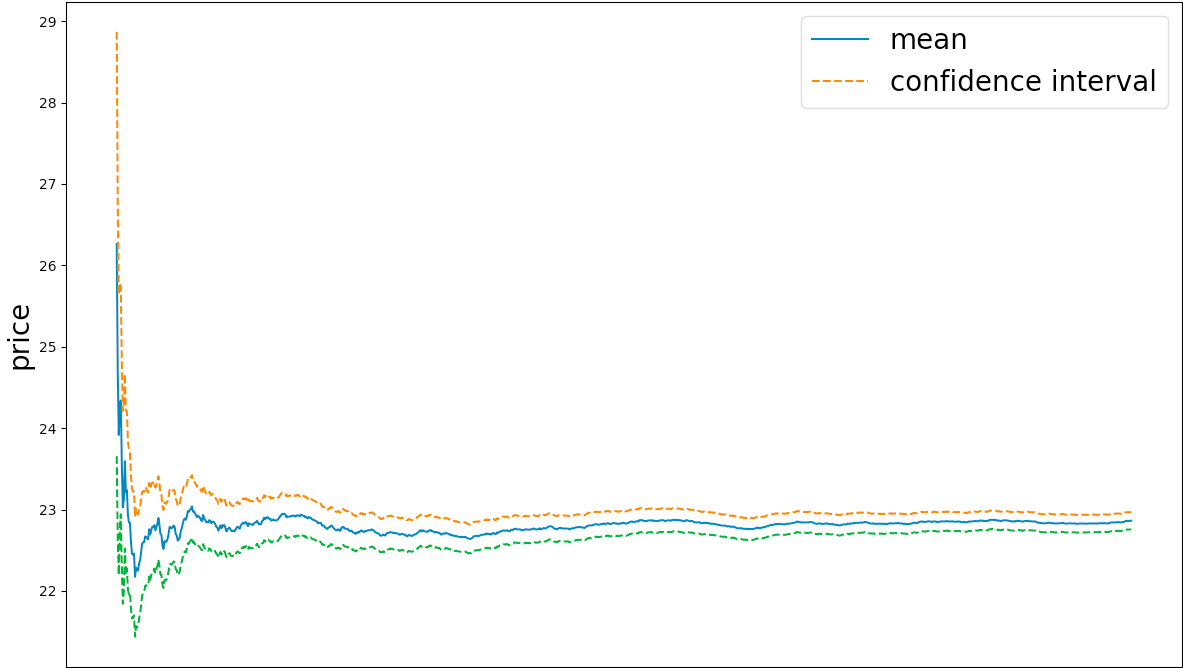
\includegraphics[width=15cm, height=6cm]{stdBasketOptionFiniteDifferenceMethodPrice.png}
				\end{figure}
			\end{center}
			
			
			\begin{center}
				\begin{figure}[!h]
					\centering
				        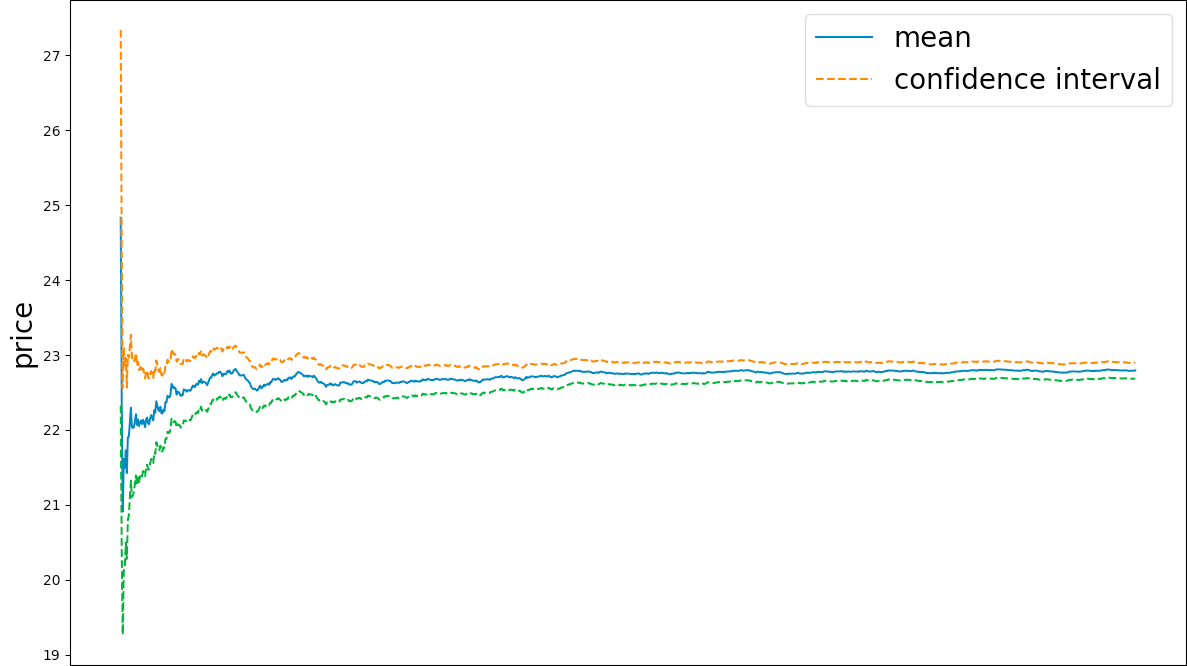
\includegraphics[width=15cm, height=6cm]{stdBasketOptionTangentModePrice.png}
				\end{figure}
			\end{center}

			\begin{center}
				\begin{figure}[!h]
					\centering
						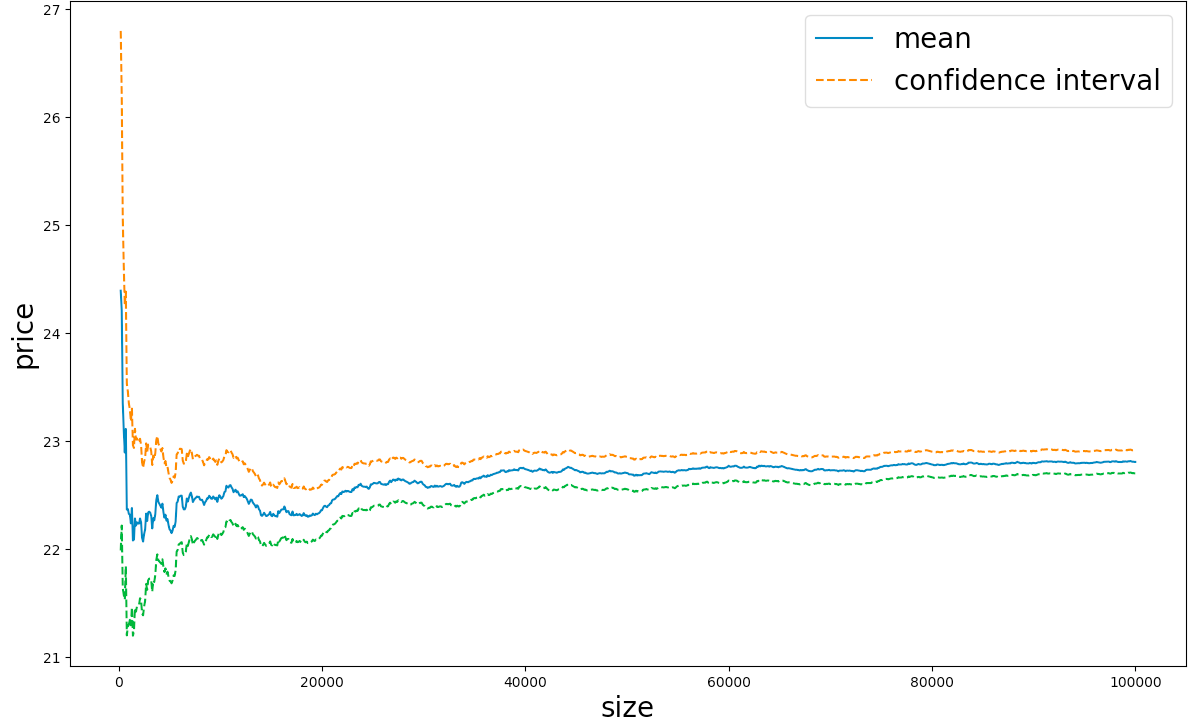
\includegraphics[width=15cm, height=6cm]{stdBasketOptionAdjointModePrice.png}
						\caption{\textbf{\underline{Basket option price using (top to bottom) finite difference method, tangent mode and adjoint mode}} 
						\\ \textit{Number of assets}: 2, \textit{Size}: $10^{5}$ samples, \textit{maturity}: 1 yr, \textit{strike}: 100, \textit{volatilities}: 30\%, \textit{initial spots}: 100, \textit{risk free rate}: 10\%, \textit{weights}: equally distributed, \textit{Correlation}: 25\%}
				\end{figure}
			\end{center}
	
			\newpage
			
			\begin{center}
				\begin{figure}[!h]
					\centering
				        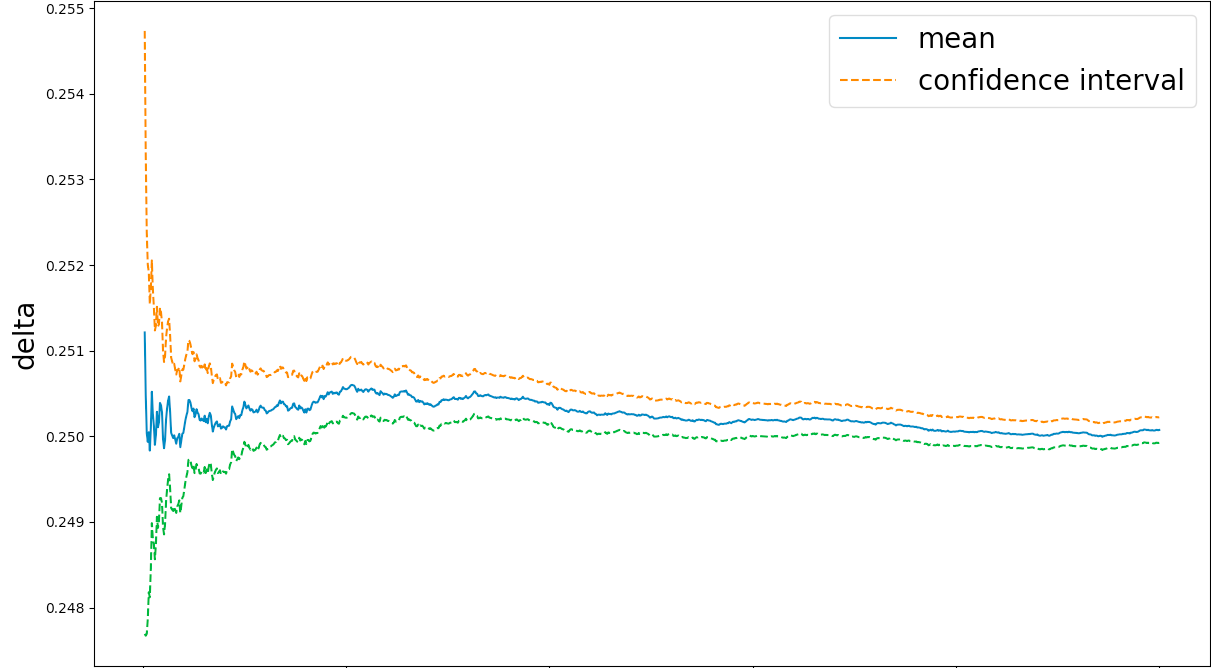
\includegraphics[width=15cm, height=6cm]{stdBasketOptionFiniteDifferenceMethodDelta.png}
				\end{figure}
			\end{center}
			
			
			\begin{center}
				\begin{figure}[!h]
					\centering
				            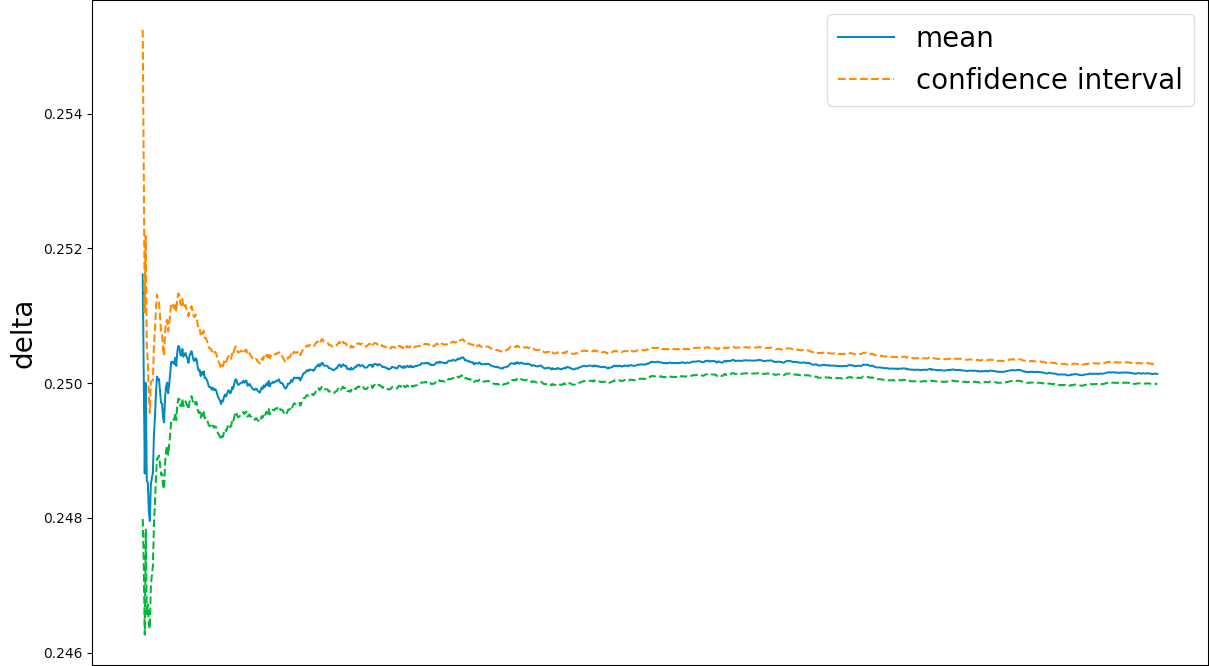
\includegraphics[width=15cm, height=6cm]{stdBasketOptionTangentModeDelta.png}
				\end{figure}
			\end{center}

			\begin{center}
				\begin{figure}[!h]
					\centering
				            \includegraphics[width=15cm, height=6cm]{stdBasketOptionAdjointModeDelta.png}
							\caption{\textbf{\underline{Basket option delta using (top to bottom) finite difference method, tangent mode and adjoint mode}} 
							\\ \textit{Number of assets}: 4, \textit{Size}: $10^{5}$ samples, \textit{maturity}: 2 yr, \textit{strike}: 95, \textit{volatilities}: 10\%, \textit{initial spots}: 120, \textit{risk free rate}: 20\%, \textit{weights}: equally distributed, \textit{Correlation}: 25\%}
				\end{figure}
			\end{center}

			\newpage

			\begin{center}
				\begin{figure}[!h]
					\centering
				            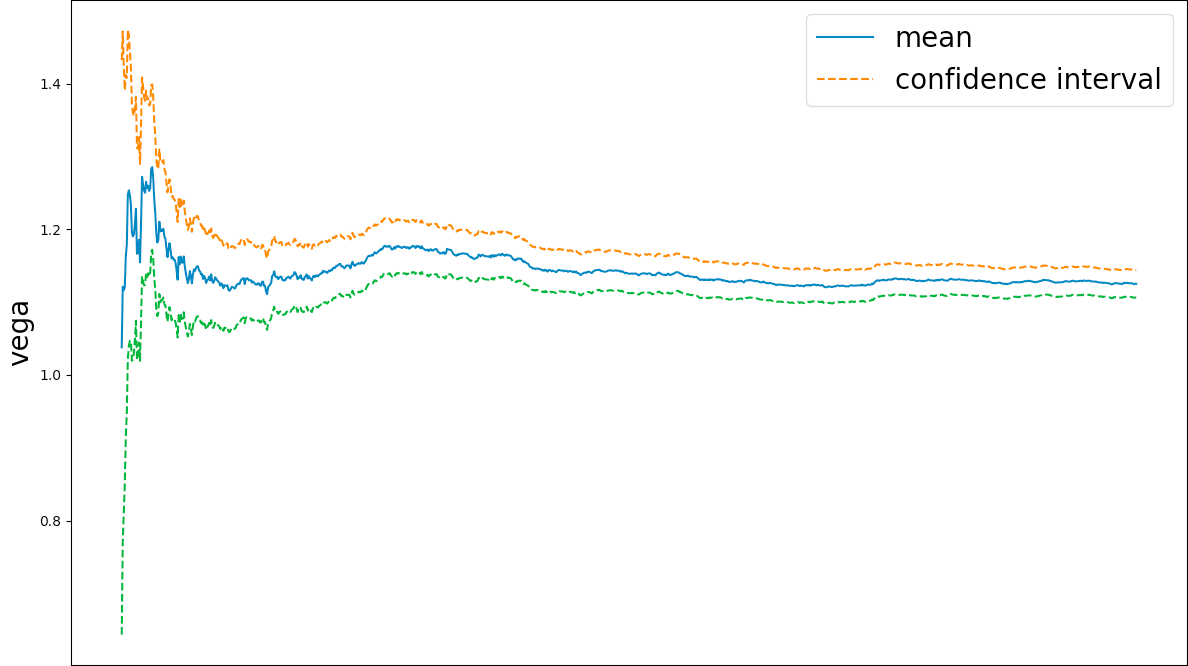
\includegraphics[width=15cm, height=6cm]{stdBasketOptionFiniteDifferenceMethodVega.png}
				\end{figure}
			\end{center}
			
			
			\begin{center}
				\begin{figure}[!h]
					\centering
				            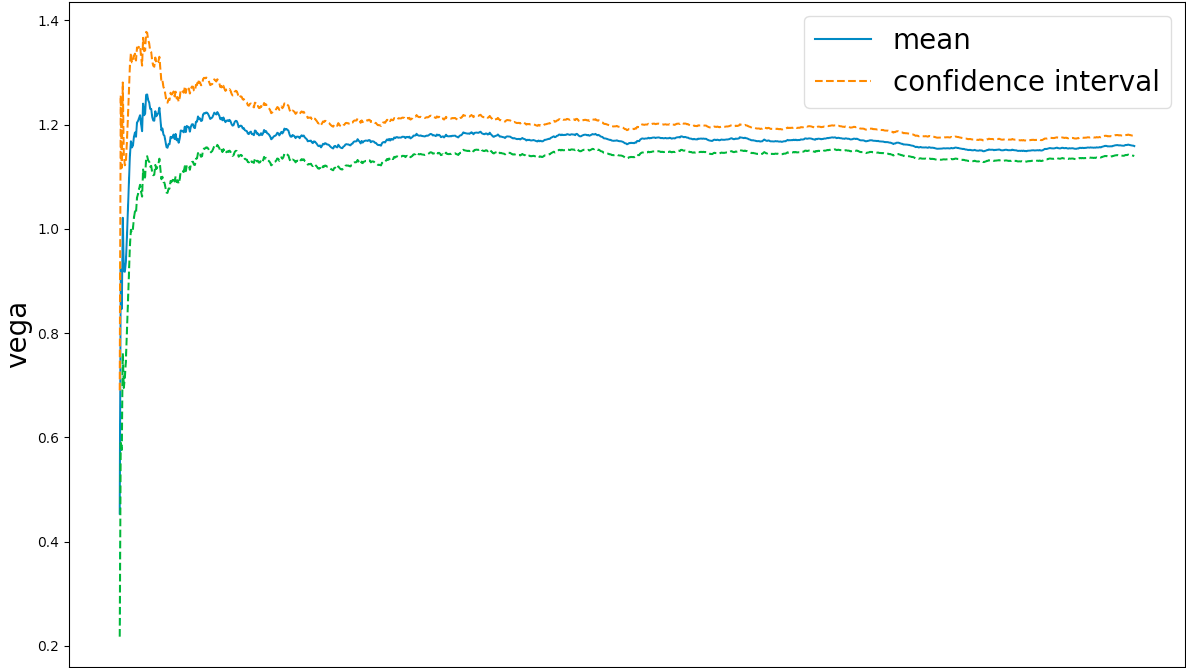
\includegraphics[width=15cm, height=6cm]{stdBasketOptionTangentModeVega.png}
				\end{figure}
			\end{center}

			\begin{center}
				\begin{figure}[!h]
					\centering
				            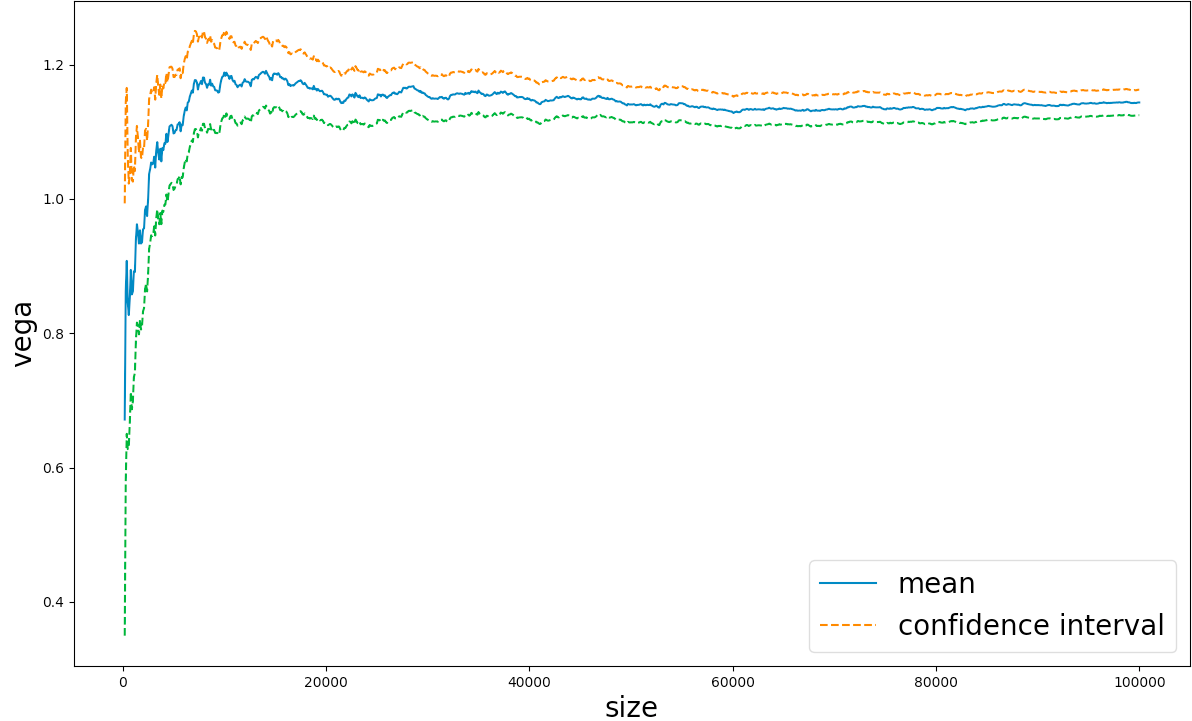
\includegraphics[width=15cm, height=6cm]{stdBasketOptionAdjointModeVega.png}
							\caption{\textbf{\underline{Basket option vega using (top to bottom) finite difference method, tangent mode and adjoint mode}} 
							\\ \textit{Number of assets}: 8, \textit{Size}: $10^{5}$ samples, \textit{maturity}: 6 mth, \textit{strike}: 110, \textit{volatilities}: 10\%, \textit{initial spots}: 100, \textit{risk free rate}: 1\%, \textit{weights}: equally distributed, \textit{Correlation}: 75\%}
				\end{figure}
			\end{center}

			\newpage

			\begin{center}
				\begin{figure}[!h]
					\centering
				            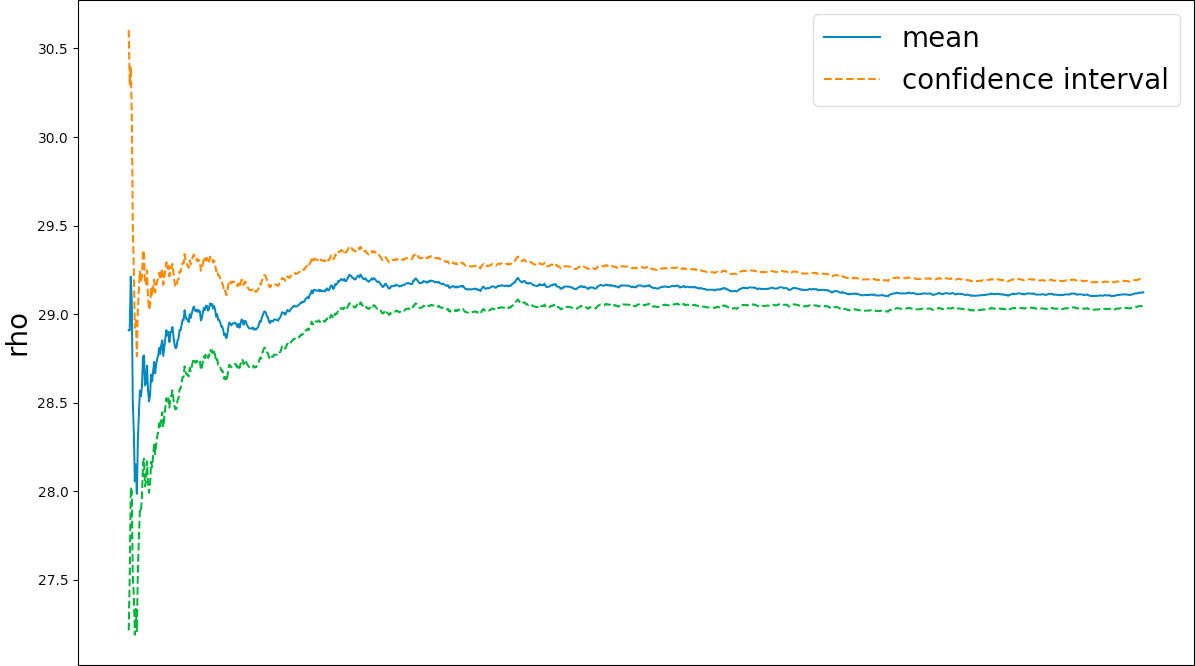
\includegraphics[width=15cm, height=6cm]{stdBasketOptionFiniteDifferenceMethodRho.png}
				\end{figure}
			\end{center}
			
			
			\begin{center}
				\begin{figure}[!h]
					\centering
				            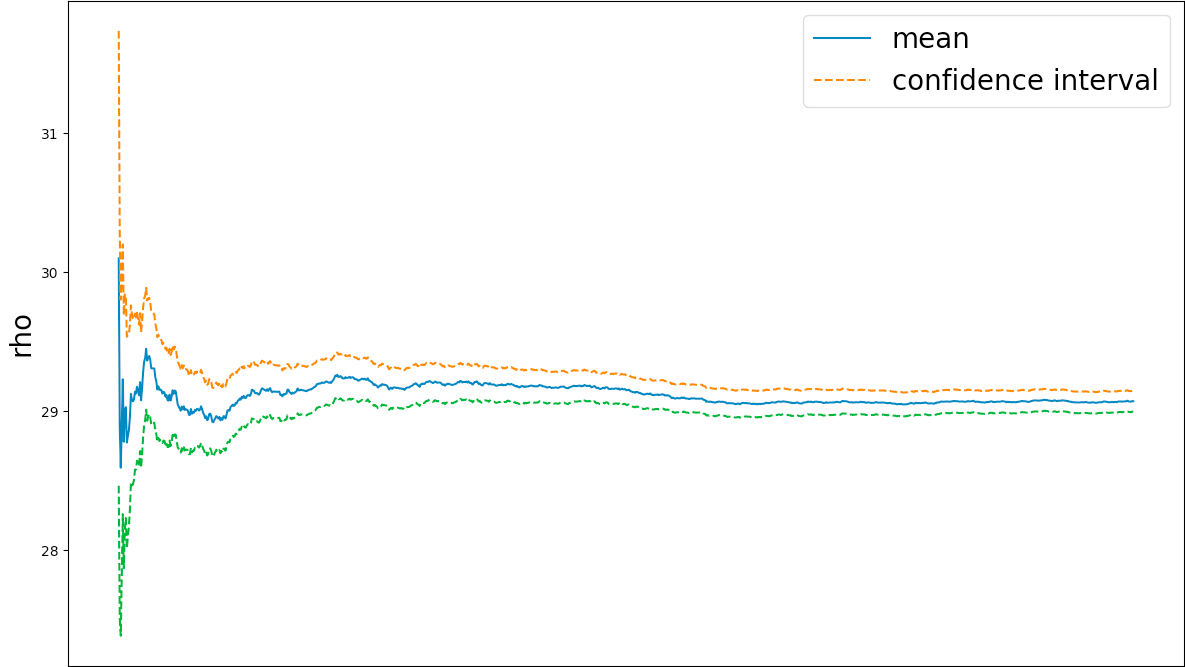
\includegraphics[width=15cm, height=6cm]{stdBasketOptionTangentModeRho.png}
				\end{figure}
			\end{center}

			\begin{center}
				\begin{figure}[!h]
					\centering
				            \includegraphics[width=15cm, height=6cm]{stdBasketOptionAdjointModeRho.png}
							\caption{\textbf{\underline{Basket option rho using (top to bottom) finite difference method, tangent mode and adjoint mode}} 
							\\ \textit{Number of assets}: 16, \textit{Size}: $10^{5}$ samples, \textit{maturity}: 3 mth, \textit{strike}: 120, \textit{volatilities}: 40\%, \textit{initial spots}: 140, \textit{risk free rate}: -1\%, \textit{weights}: equally distributed, \textit{Correlation}: 85\%}
				\end{figure}
			\end{center}

			\newpage

			The most remarquable graph of this section is the following.
			It shows clearly the power of adjoint mode versus tangent mode versus finite difference method. \\
			Indeed, one can notice that several order of magnitude in the processing time are gained.

			\begin{center}
				\begin{figure}[!h]
					\centering
							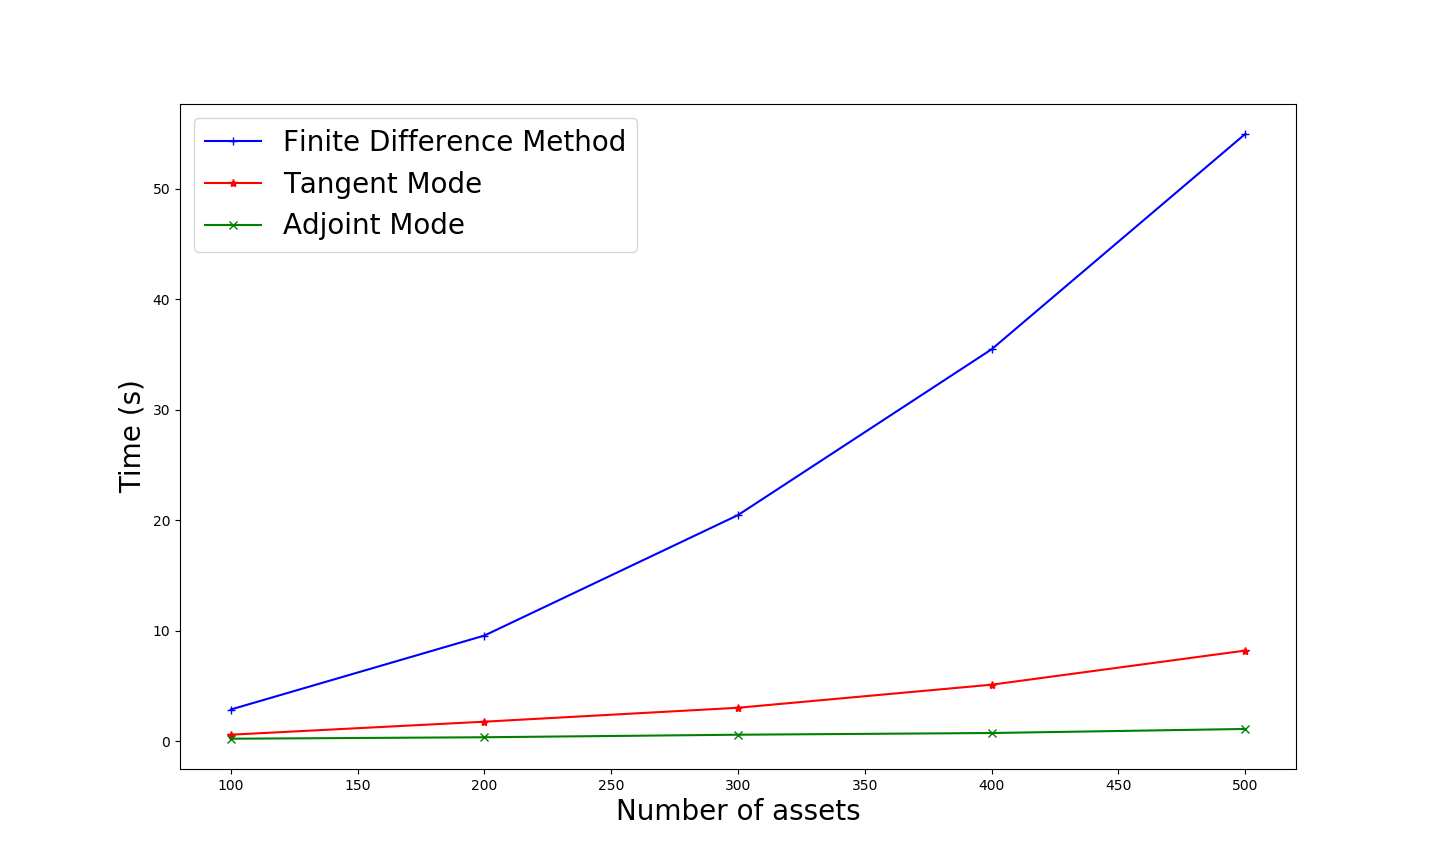
\includegraphics[width=15cm, height=10cm]{stdBasketOption.png}
							\caption{\textbf{\underline{Processing time comparison to compute basket option price, deltas, vegas and rho}} 
							\\ \textit{Number of assets}: from 100 to 500 assets, \textit{Size}: $10^{3}$ samples, \textit{maturity}: 1 yr, \textit{strike}: 100, \textit{volatilities}: 30\%, \textit{initial spots}: 100, \textit{risk free rate}: -1\%, \textit{weights}: equally distributed, \textit{Correlation}: 50\%}
				\end{figure}
			\end{center}

			\begin{center}
				\begin{tabular}{|c|c|c|c|}
					\hline
						\text{Number of assets} & \text{Finite difference method} & \text{Tangent Mode of AD} & \text{Adjoint Mode of AD} \\
					\hline
						\text{100 assets} & 2.85378s & 0.574918s & 0.210927s \\
					\hline
						200 assets & 9.55165s & 1.75251s & 0.344089s \\
					\hline
						300 assets & 20.4614s & 3.01471s & 0.573359s \\
					\hline
						400 assets & 35.4771s & 5.10348s & 0.728007s \\
					\hline
						500 assets & 54.9782s & 8.19274s & 1.09516s \\
					\hline
				\end{tabular}
			\end{center}
			
		\subsection{Best Of Asian Option}

			One now consider the case of a path-dependent option such as best of asian option.
			It consists for its holder to receive the mean of the maxima of the asset returns on fixing dates
			$0 = T_{0} < T_{1} < ... < T_{N} = T$ at price $K$, practically, the payout function writes:

			$$P(r, (x_{i,j})_{1 \leq i \leq d ; 1 \leq j \leq N}) = e^{-rT} \left( \frac{1}{N} \displaystyle{\sum_{j = 1}^{N}{\max_{i = 1 ... d}{\left(\frac{S^{i}_{T_{j}}}{S^{i}_{0}}\right)}}} - K\right)_{+}$$
		
			The advantage to work under Black-Scholes framework is that one can assume without loss of generality that $S_{0}^{i} = 1$ for all $i$,
			indeed this option is written on the returns of each asset and does not depend on the current value of the assets.

			One adds to the Black Scholes tools class a \textit{multiBlackScholes} class which produce a sample of the asset spot at the fixing dates.
			As one has built our own automatic differentiation library, there is no use to implement by hand the tangent and the adjoint mode of the payout as it is done in ~\cite{21}.
			Instead, one needs to carry out the overloading of the vector/matrix input function max and mean in each class.

			\newpage
			
			\begin{center}
				\begin{figure}[!h]
					\centering
				        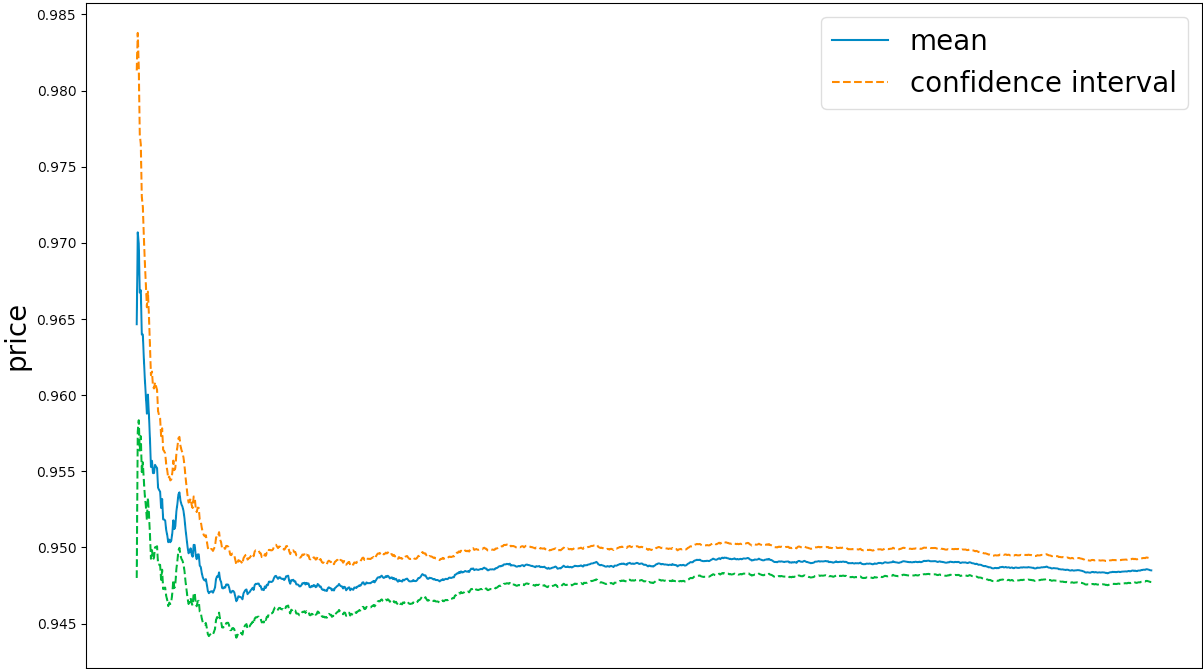
\includegraphics[width=15cm, height=6cm]{bestOfAsianOptionFiniteDifferenceMethodPrice.png}
				\end{figure}
			\end{center}
			
			
			\begin{center}
				\begin{figure}[!h]
					\centering
				        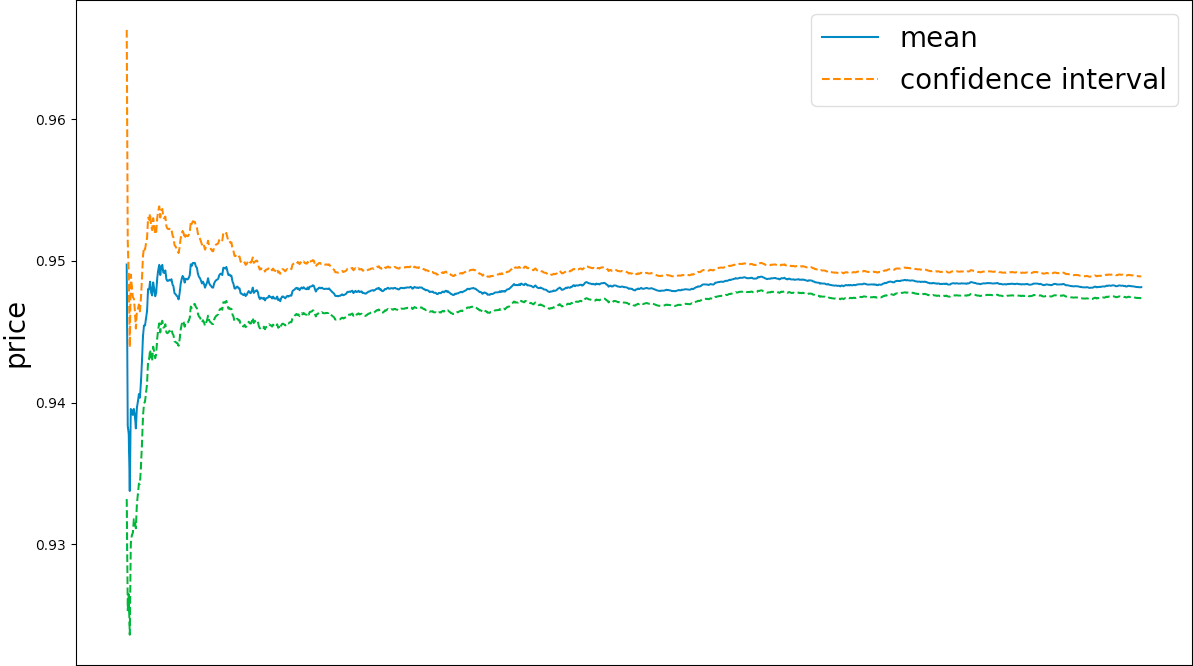
\includegraphics[width=15cm, height=6cm]{bestOfAsianOptionTangentModePrice.png}
				\end{figure}
			\end{center}

			\begin{center}
				\begin{figure}[!h]
					\centering
						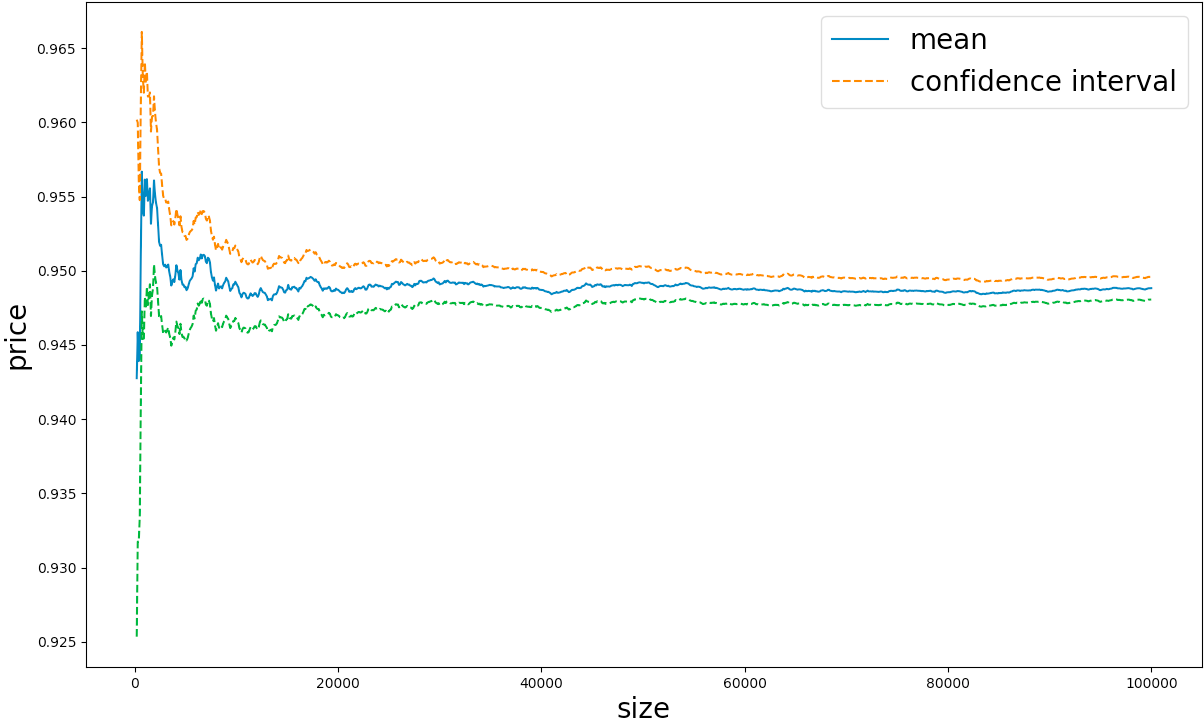
\includegraphics[width=15cm, height=6cm]{bestOfAsianOptionAdjointModePrice.png}
						\caption{\textbf{\underline{Best Of Asian Option price using (top to bottom) finite difference method, tangent mode and adjoint mode}} 
						\\ \textit{Number of assets}: 2, \textit{Fixing}: monthly, \textit{Size}: $10^{5}$ samples, \textit{maturity}: 1 yr, \textit{strike}: 1\%, \textit{volatilities}: 30\%, \textit{risk free rate}: 10\%, \textit{Correlation}: 50\%}
				\end{figure}
			\end{center}

			\newpage

			\begin{center}
				\begin{figure}[!h]
					\centering
				            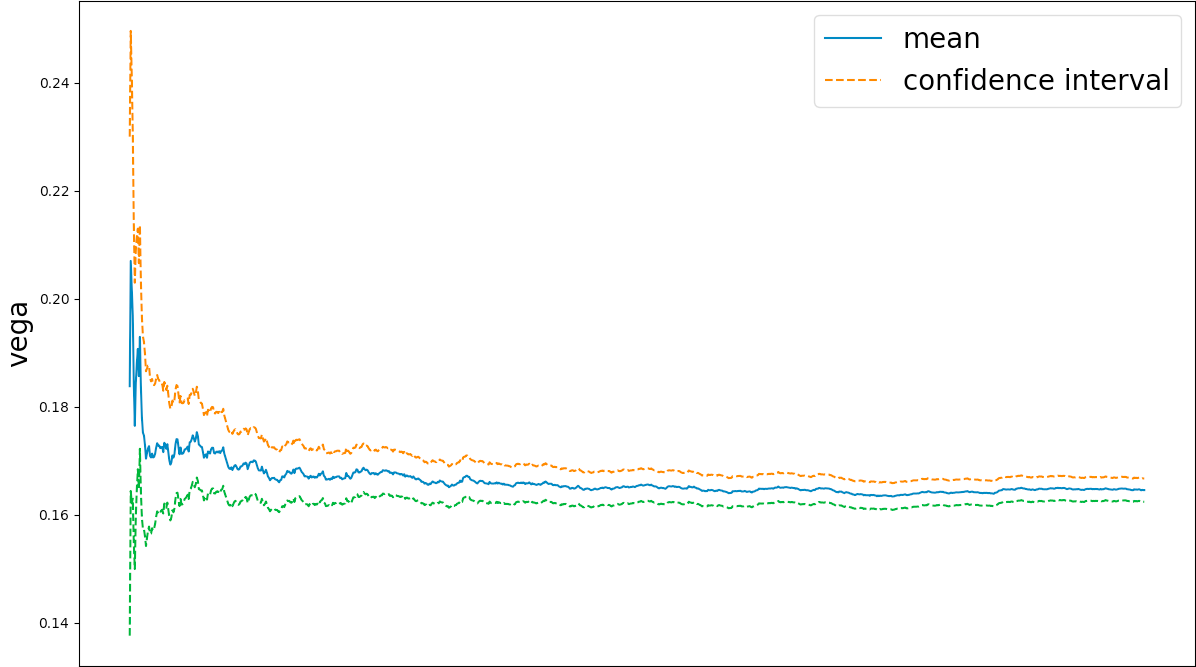
\includegraphics[width=15cm, height=6cm]{bestOfAsianOptionFiniteDifferenceMethodVega.png}
				\end{figure}
			\end{center}
			
			
			\begin{center}
				\begin{figure}[!h]
					\centering
				            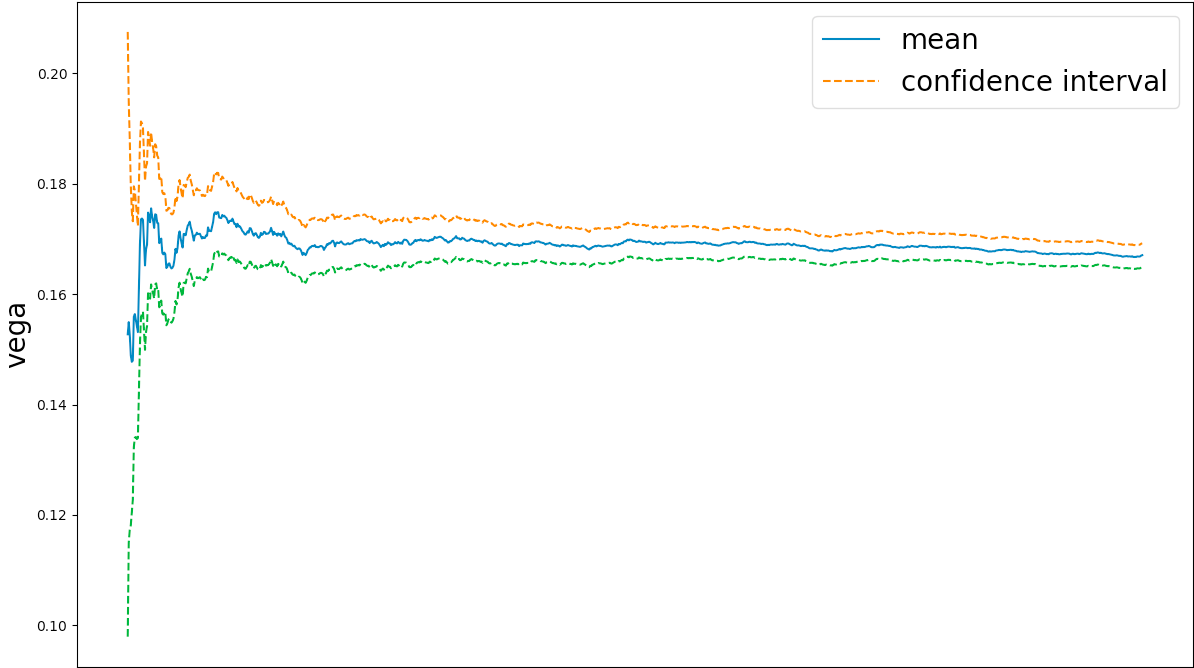
\includegraphics[width=15cm, height=6cm]{bestOfAsianOptionTangentModeVega.png}
				\end{figure}
			\end{center}

			\begin{center}
				\begin{figure}[!h]
					\centering
				            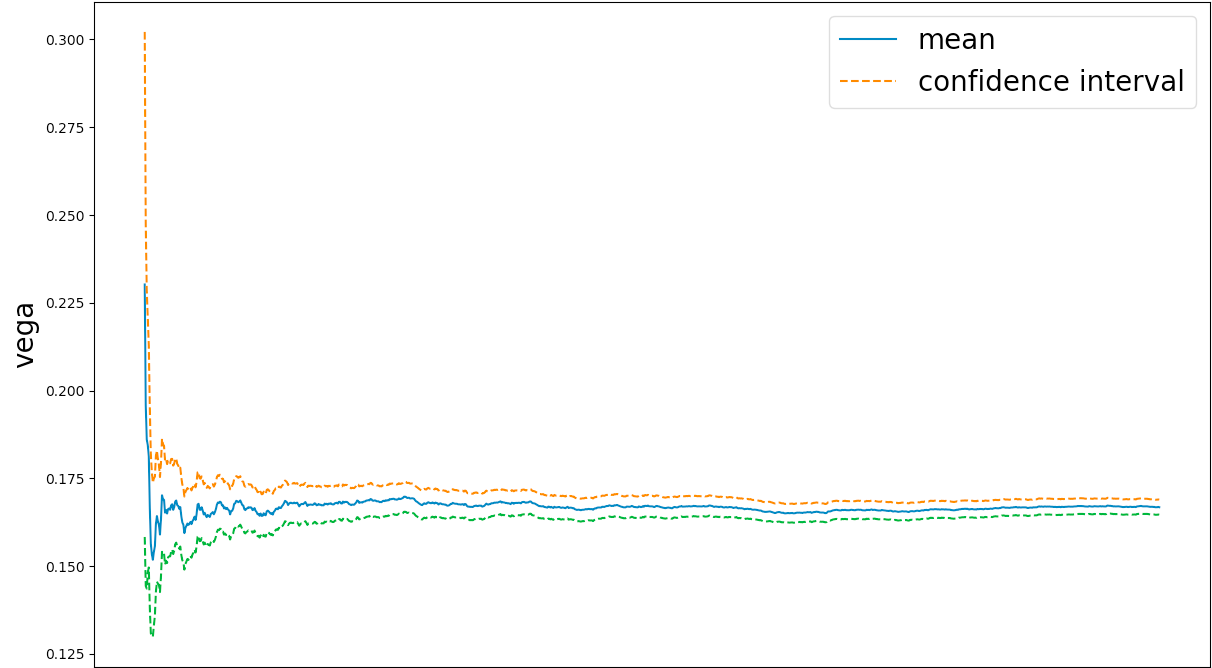
\includegraphics[width=15cm, height=6cm]{bestOfAsianOptionAdjointModeVega.png}
							\caption{\textbf{\underline{Best Of Asian option vega using (top to bottom) finite difference method, tangent mode and adjoint mode}} 
							\\ \textit{Number of assets}: 2, \textit{Fixing}: monthly, \textit{Size}: $10^{5}$ samples, \textit{maturity}: 1 yr, \textit{strike}: 1\%, \textit{volatilities}: 30\%, \textit{risk free rate}: 10\%, \textit{Correlation}: 50\%}
				\end{figure}
			\end{center}

			\newpage

			\begin{center}
				\begin{figure}[!h]
					\centering
				            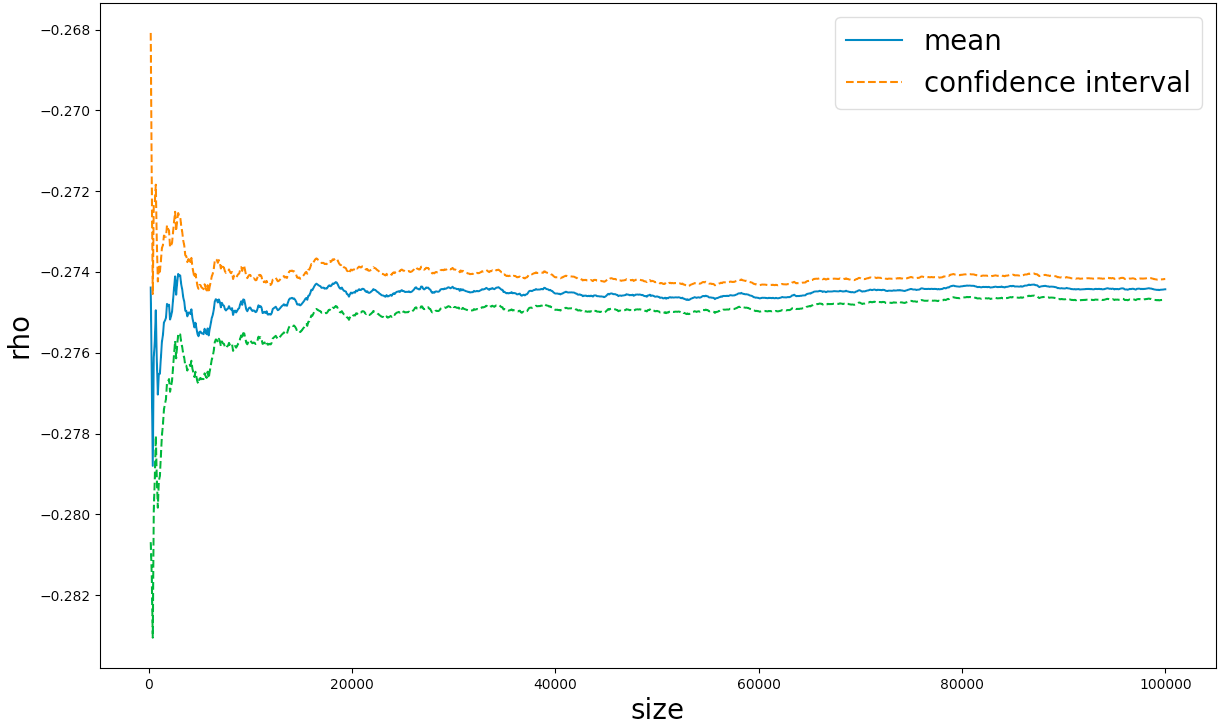
\includegraphics[width=15cm, height=6cm]{bestOfAsianOptionFiniteDifferenceMethodRho.png}
				\end{figure}
			\end{center}
			
			
			\begin{center}
				\begin{figure}[!h]
					\centering
				            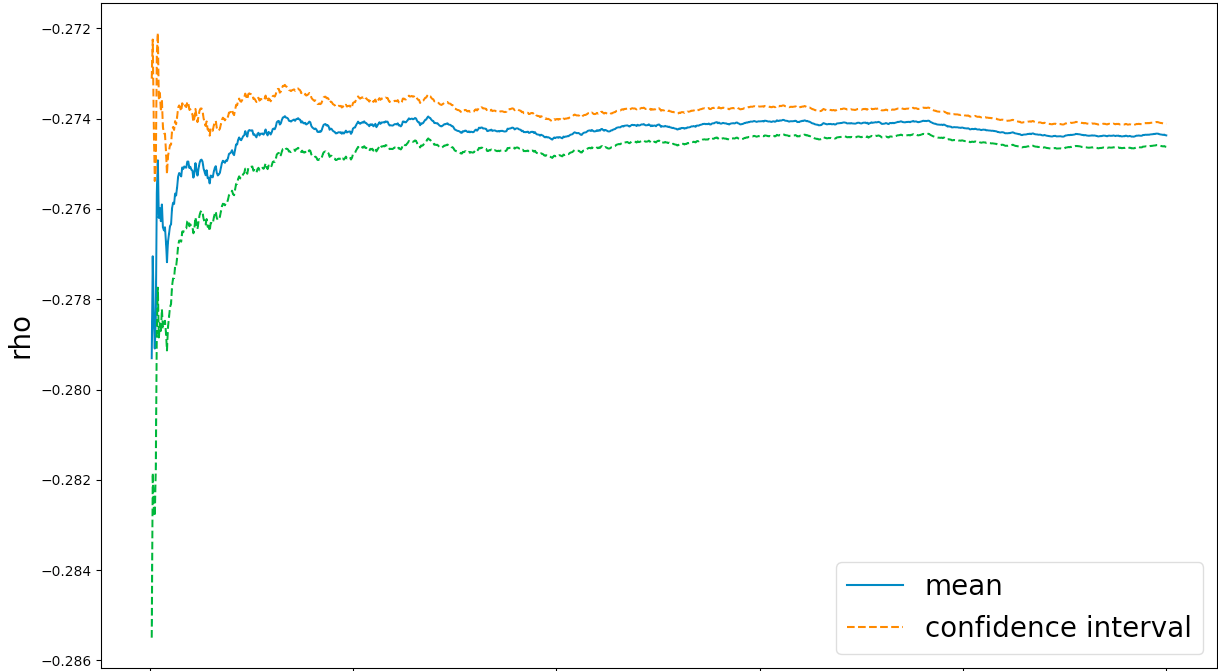
\includegraphics[width=15cm, height=6cm]{bestOfAsianOptionTangentModeRho.png}
				\end{figure}
			\end{center}

			\begin{center}
				\begin{figure}[!h]
					\centering
				            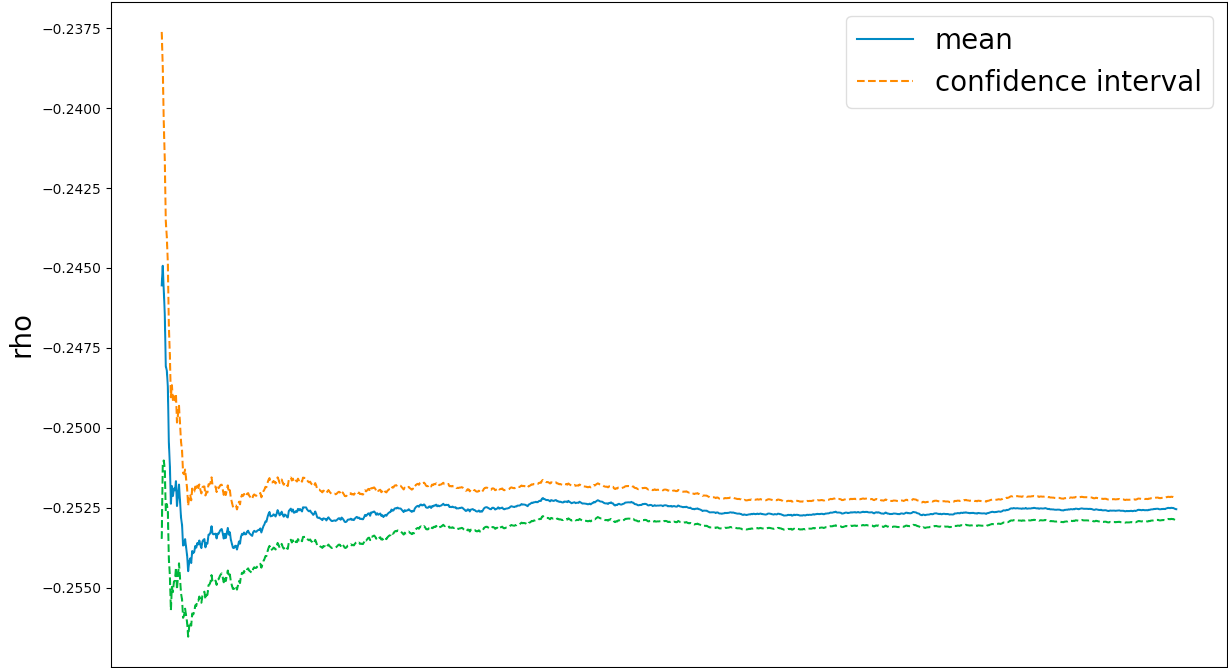
\includegraphics[width=15cm, height=6cm]{bestOfAsianOptionAdjointModeRho.png}
							\caption{\textbf{\underline{Best Of Asian Option rho using (top to bottom) finite difference method, tangent mode and adjoint mode}} 
							\\ \textit{Number of assets}: 2, \textit{Fixing}: monthly, \textit{Size}: $10^{5}$ samples, \textit{maturity}: 1 yr, \textit{strike}: 1\%, \textit{volatilities}: 30\%, \textit{risk free rate}: 10\%, \textit{Correlation}: 50\%}
				\end{figure}
			\end{center}

			\newpage

			For this kind of contingent claim, the complexity is increases linearly with $d \times N$
			when one uses finite difference method. According to the resuts presented below, adjoint mode of AD 
			holds highly accurate and speed compare to others and one notices that for large number of assets, it becomes
			the main tool to produce results quickly. 

			\begin{center}
				\begin{figure}[!h]
					\centering
							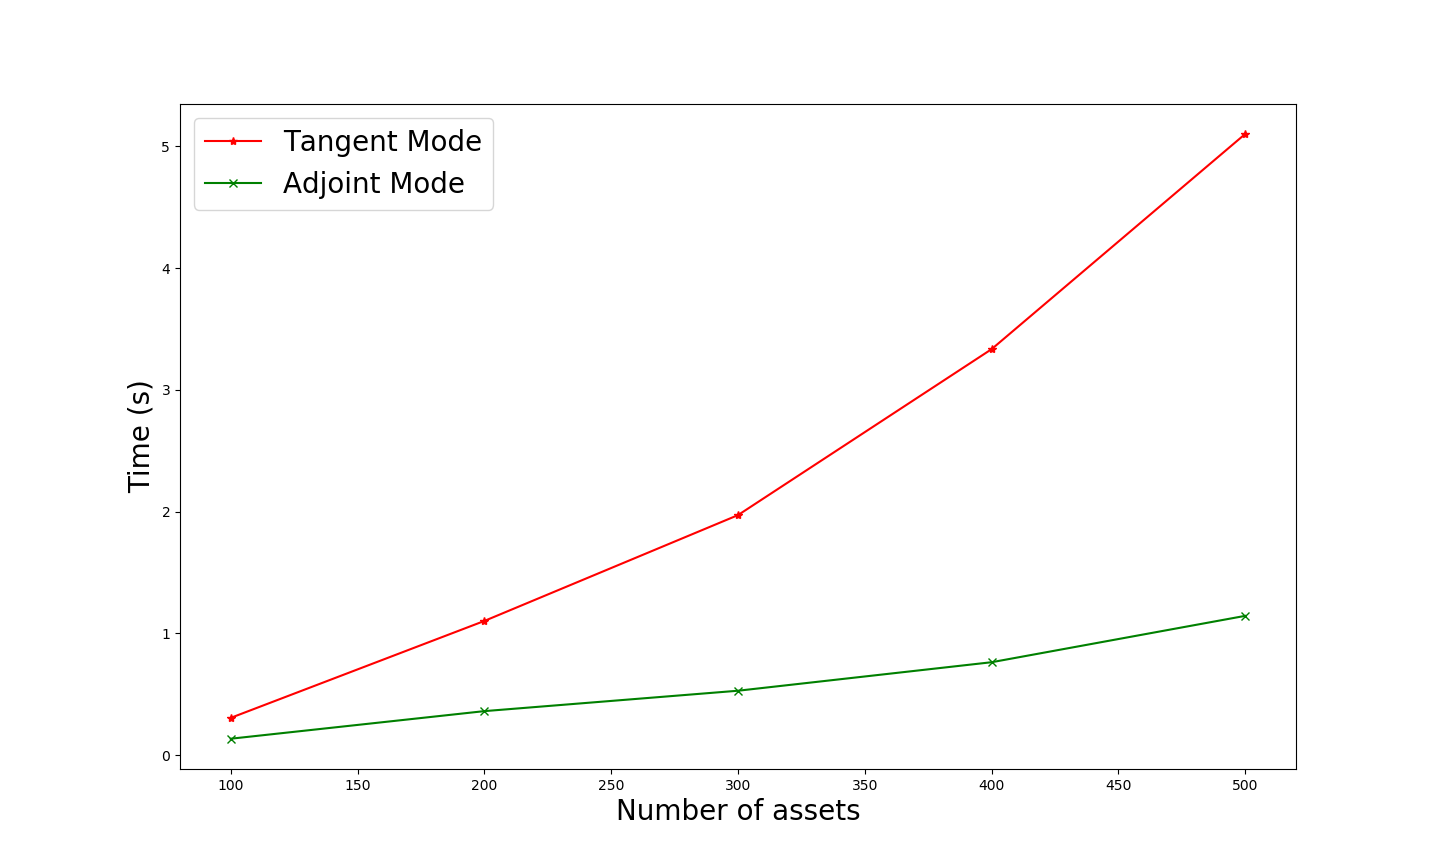
\includegraphics[width=15cm, height=10cm]{bestOfAsianOption.png}
							\caption{\textbf{\underline{Processing time comparison to compute best of asian option price, vegas and rho}} 
							\\ \textit{Number of assets}: from 100 to 500, \textit{Fixing}: monthly, \textit{Size}: $10^{5}$ samples, \textit{maturity}: 1 yr, \textit{strike}: 1\%, \textit{volatilities}: 30\%, \textit{risk free rate}: 10\%, \textit{Correlation}: 50\%}
				\end{figure}
			\end{center}

			\begin{center}
				\begin{tabular}{|c|c|c|c|}
					\hline
						\text{Market parameters} & \text{Finite difference method} & \text{Tangent Mode of AD} & \text{Adjoint Mode of AD} \\
					\hline
						\text{Price} & 1.04858 & 1.05031 & 1.0492 \\
					\hline
						$\gamma_{1}$ & 0.1638 & 0.1673 & 0.1662 \\
					\hline
						$\gamma_{2}$ & 0.1668 & 0.1691 & 0.1670 \\
					\hline
						$\rho$ & -0.252635 & -0.274637 & -0.274441 \\
					\hline
				\end{tabular}
			\end{center}

			\begin{center}
				\begin{tabular}{|c|c|c|c|}
					\hline
						\text{Number of assets} & \text{Finite difference method} & \text{Tangent Mode of AD} & \text{Adjoint Mode of AD} \\
					\hline
						100 assets & 28.0003s & 0.306534s & 0.135332s \\
					\hline
						200 assets & 110.797s & 1.10229s & 0.361844s \\
					\hline
						300 assets & 247.113s & 1.97121s & 0.529366s \\
					\hline
						400 assets & 457.815s & 3.33394s & 0.763426s \\
					\hline
						500 assets & 702.954s & 5.10094s & 1.14418s \\
					\hline
				\end{tabular}
			\end{center}
			
	\section{Correlation greeks}

		One decides to make the correlation sensitivities computation in another framework.
		Here, one seeks to use automatic differentiation tools to compute the correlation part of the tangent state vector.
		It involves the calculation of the adjoint of cholesky decomposition.
		In ~\cite{22}, the author implement it by hand but one can proceed in an automatic way as one built the structure to do so.

		\begin{center}
			\begin{figure}[!h]
				\centering
						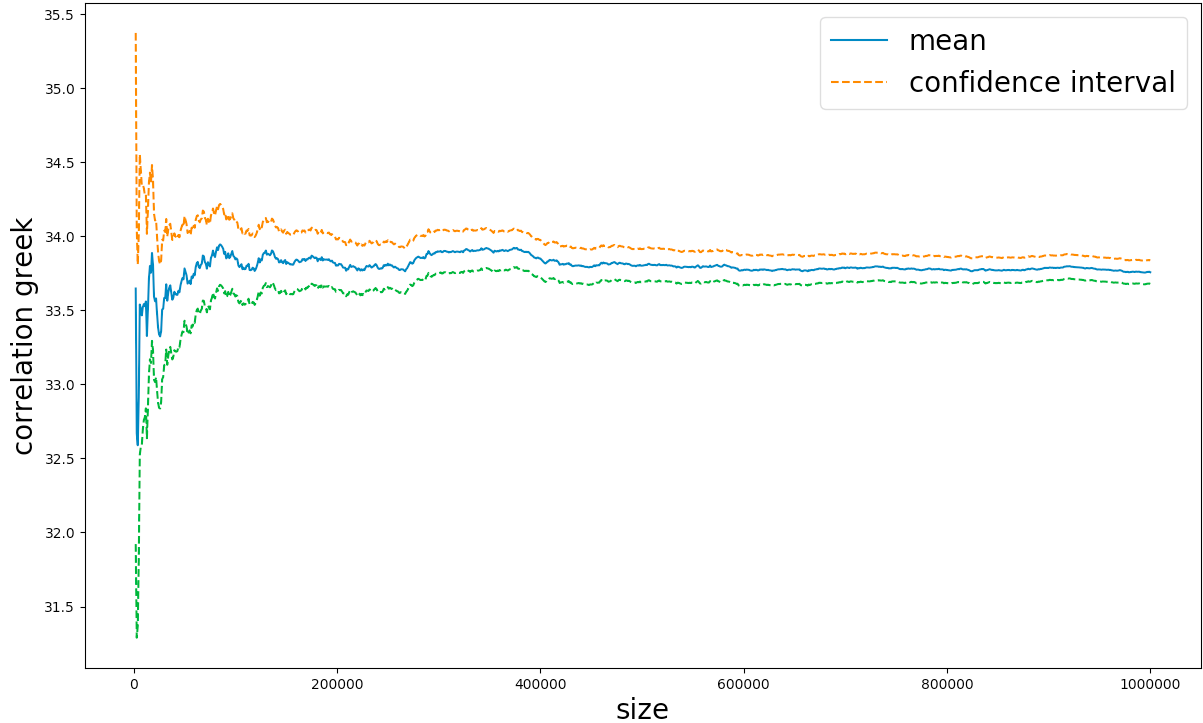
\includegraphics[width=15cm, height=10cm]{correlationShow.png}
						\caption{\textbf{\underline{Basket Option correlation sensitivity}} 
						\\ \textit{Number of assets}: 2, \textit{Size}: $10^{5}$ samples, \textit{maturity}: 1 yr, \textit{strike}: 100, \textit{volatilities}: 30\%, \textit{initial spots}: 100, \textit{risk free rate}: 10\%, \textit{weights}: equally distributed, \textit{Correlation}: 25\%}
						
			\end{figure}
		\end{center}

		\begin{center}
			\begin{figure}[!h]
				\centering
						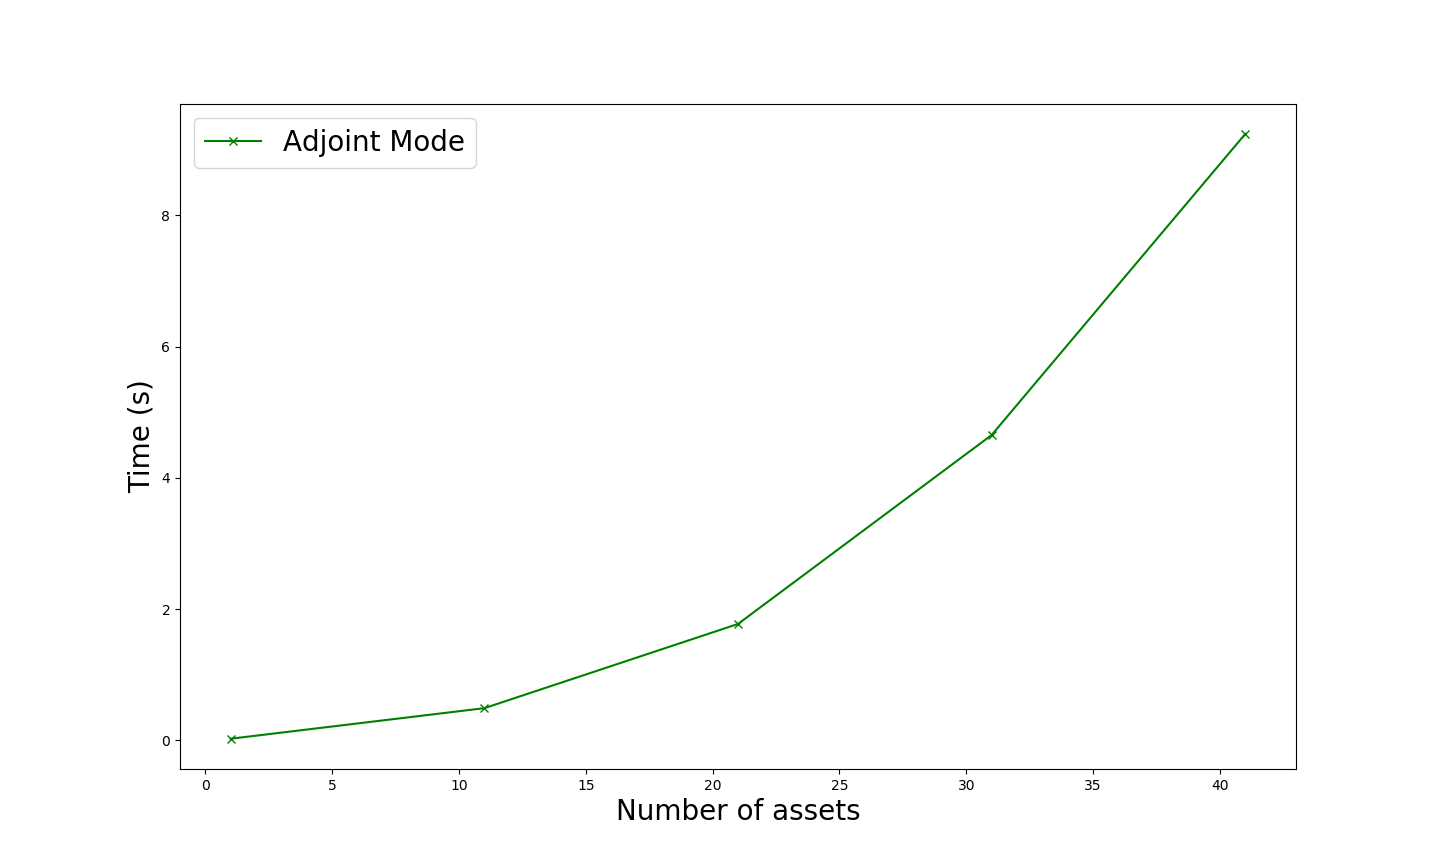
\includegraphics[width=15cm, height=10cm]{correlationTime.png}
						\caption{\textbf{\underline{Processing time comparison to compute basket option correlation greeks}} 
						\\ \textit{Number of assets}: from 100 to 500, \textit{Fixing}: monthly, \textit{Size}: $10^{5}$ samples, \textit{maturity}: 1 yr, \textit{strike}: 1\%, \textit{volatilities}: 30\%, \textit{risk free rate}: 10\%, \textit{Correlation}: 50\%}
			\end{figure}
		\end{center}
	
	\section{Conclusion}
	
		In this short report, I was seeking to explain as clearly as possible how algorithmic differentiation works
		and shows throughout simple examples of correlation products its efficiency and in particular the power of adjoint mode,
		which provides several orders of magnitude and speeds significantly the greeks calculation.
		I hope I have conviced the reader to use this technology in its future implementation works.
		As further works, one can apply it to the computation of the tangent state vector under more complex model with for example,
		given a diffusion scheme, seeking to diffuse the derivatives of the state vector with respect to the parameters involved.

	\listoffigures

	\bibliographystyle{plain}
	\bibliography{greeksComputationWithAlgorithmicDifferentiationLibrary}	

\end{document}